\documentclass[%
xelatex,
	oneside,		% Single side print
	12pt,			% Font size
	parskip=half,	% Half line skip between paragraphs
%	headsepline,	% Line after header
%	footsepline,	% Line before footer
	abstracton,
	chapterprefix=true% like in standard class "report"
    appendixprefix=true]
{scrbook}
\usepackage[english]{babel}

\usepackage{rwukoma}
\usepackage[pdfusetitle]{hyperref}
\title{Master Thesis}
\author{Viplav Setia}
\usepackage{graphicx}
\usepackage{nomencl}
\makenomenclature
\renewcommand{\nomname}{List of abbreviations, formulas and indexes}
\usepackage{blindtext}
\usepackage{caption}
\usepackage{scrlayer-scrpage}
\pagestyle{scrheadings}
\clearscrheadfoot
\rofoot{\pagemark}
\refoot{\pagemark}
\automark{chapter}
\ohead{\headmark}
\setlength{\nomlabelwidth}{2cm}
\setlength{\nomitemsep}{-\parsep}
\usepackage{hyperref}
\usepackage{amssymb}
\usepackage{siunitx}

\begin{document}

\section*{\Large\normalfont\bfseries Declaration}
	\addcontentsline{toc}{chapter}{Declaration}

I, Viplav Setia, born on 04.04.1995 in New Delhi, India, assure that I have done this work independently. All sources and references used for the completion of this
thesis have been listed and cited accordingly. This thesis work was done in
partial fulfillment of the requirements for the award of the degree of Master of
Science in Mechatronics at Hochschule Ravensburg Weingarten and has not been
used or submitted elsewhere for award of a degree, grade or in any publication. \newline


\rule{5cm}{.4pt}

Viplav Setia \newline
Friedrichshafen, 31 January 2020
\clearpage

		\section*{\Large\normalfont\bfseries Acknowledgement}
		\addcontentsline{toc}{chapter}{Acknowledgement}

I would like to express my heartfelt
gratitude to Prof Dr.-Ing Benedikt Reick and Prof Dr. rer. nat. Markus Pfeil for guiding me through the completion of my Master thesis and for their valuable
suggestions.

I am extremely thankful to ALTEN GmbH and their colleagues who gave me this opportunity and the resources to do this thesis at their office branch in Friedrichshafen. They also supported me with their knowledge,  expertise and created a pleasant working environment, without which it would have been difficult to move forward with this project.

Also, many thanks to my family and friends for their constant encouragement.				
	\clearpage
		\section*{\Large\normalfont\bfseries Abstract}
		\addcontentsline{toc}{chapter}{Abstract}

The automotive industry is changing rapidly to new technologies like electromobility and automated driving. All major companies in the automotive sector are investing heavily to bring electric cars to the market and develop prototypes for automated driving. To support this change, middleware is required which is used as a means of data exchange between various sensors, control systems and actuators. The focus of this thesis is to test the new versions of the middleware, Robot Operating System (ROS\nomenclature{ROS}{Robot Operating System}), which offer support for embedded and real-time systems. Additionally, a model using the Gazebo robot simulator was developed to explore \nomenclature{ADAS}{Advanced Driver Assistance Systems} Advanced Driver Assistance Systems (ADAS) applications using a camera and a Light Detection and Ranging (LIDAR)\nomenclature{LIDAR}{Light Detection and Ranging} sensor as an example to show the data transfer using ROS 2 for the automotive industry. To test the real-time performance of ROS2, an inverted pendulum demo was used and its simulation was visualized on a Linux system enabled with real-time capabilities. To test the reliability of the version micro-ROS, a demonstrator was built using a STM32 microcontroller with Nuttx Real-Time Operating System (RTOS\nomenclature{RTOS}{Real-Time Operating System}) installed to show the data transfer of a pressure sensor. To test the real-time performance for this version, an algorithm was created to test the delay in data transfer with different data sizes. Finally, the results were analyzed and discussed which also helped in suggesting future research scope.
\clearpage

	\addcontentsline{toc}{chapter}{List of abbreviations, formulas and indexes}
	
\rofoot[\pagemark]{\pagemark}
\refoot[\pagemark]{\pagemark}
\printnomenclature
	

	\tableofcontents
	
	


	\chapter{Introduction}

\rofoot[\pagemark]{\pagemark}
\refoot[\pagemark]{\pagemark}

A modern car is a complex assembly of all kinds of sensors, control systems, actuators, drives and mechanical components. A great amount of data is flowing between different components of a car which needs to be managed and also arrive at the right place at the right time. As shown in figure 1.1, Intel suggests about 4000 gigabytes (GB) of data flow per day will take place in the future. Therefore, research and testing of real-time software is important in the automotive domain. The motivation to do it and the way it has been done in this thesis work is described in this chapter. Also, a brief introduction to ROS and its version is stated. 
\nomenclature{GB}{Gigabytes}
\begin{center}
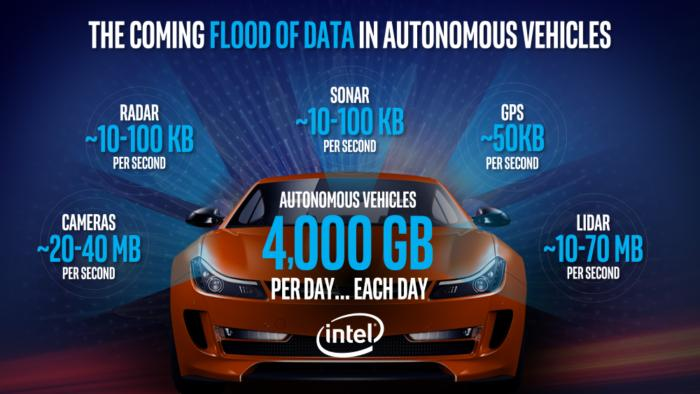
\includegraphics[scale=.5]{fig/autonomous-vehicle-data-intel-100697604-large.jpg}
\captionof{figure}[Data Stats in Autonomous Cars]{Data Stats in Autonomous Cars \cite{datastats}}
\label{fig:datastats}
\end{center}

     \section{Motivation}	
For automotive applications, one major challenge is that all systems in the car should be real-time safe, that is, all systems of the car must give a guaranteed response within a specified time constraint. Missing a deadline can have disastrous consequences, such as, failure to apply the brakes at the right time after recognizing a person in front of the car may result in loss of life. 
One such software for communication data management is ROS. New versions of ROS, namely, ROS 2 and micro-ROS offer support for real-time systems and embedded boards. The goal of this thesis is to test the real-time capability and robustness of ROS 2 and micro-ROS under different test conditions.
	 \section{Objectives}
The objective is to explore the differences between ROS and its new versions ROS 2 and embedded based micro-ROS and establish their working environments on a Linux machine and a microcontroller respectively to test their functionality and real-time performance.


In this thesis work, an overview of the state of the art in the fields of ROS 2 software development, micro-ROS architecture, embedded hardware and communication protocols used with ROS 2, real-time systems, and available research of real-time testing of ROS 2 has been documented. 

To explore ADAS applications and apply the concepts of ROS 2, a model with camera and LIDAR sensor was built in Gazebo robot simulator. Real-time testing of ROS 2 was done with the inverted pendulum demo package. 

The next step was to set up the micro-ROS environment with RTOS on a STM32 microcontroller. Micro-ROS was tested for reliability and real-time capability. Finally, the results were analyzed and future research work has been suggested.

	 \section{Robot Operating System (ROS)}
	 
Different versions of ROS are available and are under development for different kinds of applications. They are:

	 
	 {\bfseries ROS}
	 
"ROS is a flexible framework for writing robot software. It is a collection of tools, libraries, and conventions that aim to simplify the task of creating complex and robust robot behaviour across a wide variety of robotic platforms." \cite{ROS}	
It is an open-source software and is free to use for both research and commercial purposes.
 
 \nomenclature{CPU}{Central Processing Unit}
In addition, the ROS cannot guarantee deadlines (response within a specified time constraints). Moreover, the ROS requires significant resources (e.g, CPU, memory, network bandwidth) and cannot manage these resources to meet time constraints. Therefore, ROS is not suitable for real-time embedded systems.\cite{rosvsros2}
\clearpage
{\bfseries	 ROS 2}

ROS 2 was developed to satisfy new use cases like real-time systems, embedded systems, non-ideal networks, and production environments. It also uses new technologies like Data Distribution Service (DDS)\nomenclature{DDS}{Data Distribution Service}. The software is developed and maintained by Open Robotics.
It also offers support for different operating systems such as Linux, macOS, Microsoft Windows and different RTOSs. 

{\bfseries	 ROS 2 Distributions}
	 

The ROS 2 Distributions are shown in figure 1.2 in descending order of release date. Dashing Diademata is the first long term support version offered by the ROS developers. The work in this thesis is based on the versions Crystal Clemmys and Dashing Diademata. Dashing version release states that it is an improvement over the Crystal version especially for using less memory during runtime which helps in achieving better real-time performance. 

 
\includegraphics[scale=0.85]{fig/ros2distro.png}
\captionof{figure}[ROS 2 Distributions]{ROS 2 Distributions \cite{ROS2distro}}
\label{fig:ROS2Distro}

\vspace*{1cm}

{\bfseries Micro-ROS}
\vspace*{0.5cm}

"Micro-ROS puts ROS 2 onto microcontrollers, making them first class participants of the ROS 2 environment." \cite{uros}	
It uses a RTOS - Nuttx by default, and DDS for eXtremely Resource Constrained Environments (DDS-XRCE)\nomenclature{DDS-XRCE}{DDS for eXtremely Resource Constrained Environments}. In this thesis, ROS 2 Crystal version is used with Nuttx RTOS on a STM32 microcontroller which is a 32-bit microcontroller by STMelectronics. The micro-ROS project is funded by Open Framework for Embedded Robot Applications (OFERA)\nomenclature{OFERA}{Open Framework for Embedded Robot Applications} consortium consisting of Bosch, eProsima, Acutronic Robotics, FIWARE, and PIAP. Figure 1.3 shows the official logo of micro-ROS.

\begin{figure}[ht]
\begin{center}

\includegraphics[scale=.3]{fig/microROS-big-logo.png}
\caption[micro-ROS Logo]{micro-ROS Logo \cite{uroslogo}}
\label{fig:uros}
\end{center}
\end{figure} 
	 
	\chapter{State of the Art}	

\rofoot[\pagemark]{\pagemark}
\refoot[\pagemark]{\pagemark}
The core concepts of ROS 2, micro-ROS, used embedded hardware, used communication protocols and real-time systems are described in this chapter.

Real-time applications of ROS 2 have very recently come into the picture. Developers at Bosch, ApexAI, and Nobleo Technology have tested ROS 2 and have identified problems related to real-time performance which are mentioned in the section - "Available Research on Real-Time Testing of ROS 2". Also, the micro-ROS project is still in its beginning stage.
 
	\section{ROS 2 Concepts}
	
	\vspace*{0.5cm}
	In this section, the communication framework of ROS 2 is defined. Different layers of the software and their working is described in brief.
	
	
	\vspace*{0.5cm}
	{\bfseries Node}
	
	
	\vspace*{0.5cm}
An executable/application which communicates via streaming topics is known as a node.
It is used to communicate with other nodes using ROS client libraries which allow nodes to be written in different programming languages such as C, C++ and python. A robot may contain multiple nodes to control movement, analyze data, and perform an operation like path planning.

In ROS 2, discovery of nodes is automatic through the underlying middleware. Nodes advertise information to other nodes when they go online, offline and also periodically for new nodes to join and enable communication. 

ROS 2 design introduces the concept of node lifecycle, which helps to separate the real-time code path from the non real-time tasks. All memory allocations are done during node initialization which are the non real-time tasks, and then the real-time tasks (e.g. - calculations, data exchange, and data processing) take place. 


\vspace*{0.4cm}
	{\bfseries Topic}
	
	
	\vspace*{0.4cm}
	"Topics are named buses over which nodes exchange messages. Topics have anonymous publish/subscribe semantics, which decouples the production of information from its consumption. In general, nodes are not aware of the other nodes they are communicating with. Instead, nodes that are interested in data subscribe to the relevant topic and nodes that generate data publish to the relevant topic. There can be multiple publishers and subscribers to a topic." \cite{topic}
\clearpage
	{\bfseries Message}
	
	
	\vspace*{0.5cm}
A message is a simple data structure, comprising typed fields. Standard primitive types (e.g. - integer, floating point, and boolean) are supported, as well as arrays of primitive types. For specifying the data structure of a message, simple text files are used which are known as msg (message) files. These files are stored in the msg (message) subdirectory of a package. The request and response messages which are part of a ROS service call are defined in srv (service) files which are stored in the srv subdirectory of a package. Nodes communicate with each other by publishing messages to topics.\cite{messages}


	\vspace*{0.25cm}
In figure 2.1, the working of ROS 2 communication is shown. The nodes can be independently created in different programming languages. For example, a laser scanner node created with Python publishes data to the topic "Laser Data" which is subscribed by a map building node created with C++. 
\begin{center}
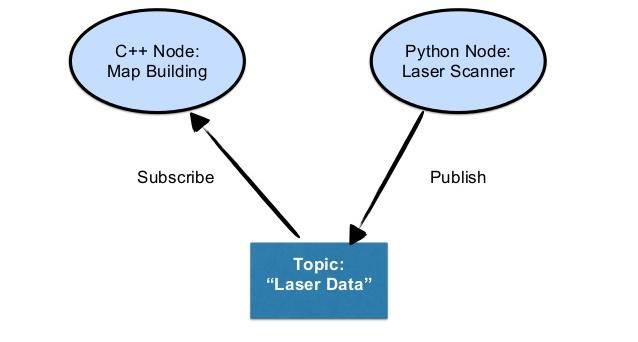
\includegraphics[scale=0.7]{fig/node_topic.jpg}
\captionof{figure}[Working of Nodes, Topics and Messages]{Working of Nodes, Topics and Messages \cite{node_topic}}
\label{fig:node}
\end{center}


\vspace*{0.25cm}

	{\bfseries Data Distribution Service (DDS)}
	
	
	\vspace*{0.5cm}
	DDS is a middleware standard that provides discovery, serialization (breaking down of data into small packets), and transportation to ensure dependable, real-time, and interoperable data exchanges.
	In a distributed system, the software layer that lies between the operating system and applications is known as middleware. "It enables the various components of a system to more easily communicate and share data. It simplifies the development of distributed systems by letting software developers focus on the specific purpose of their applications rather than the mechanics of passing information between applications and systems." \cite{DDS}


	\vspace*{0.25cm}
In figure 2.2, the different layers in a distributed system have been described. The application or node developer does not need extensive knowledge about the underlying middleware schemantics, serialization, transportation and prioritization of data exchanges. The developer can use the application packages depending on the communication protocols and data types defined in the user manual of ROS 2 to create the application.	
\begin{center}
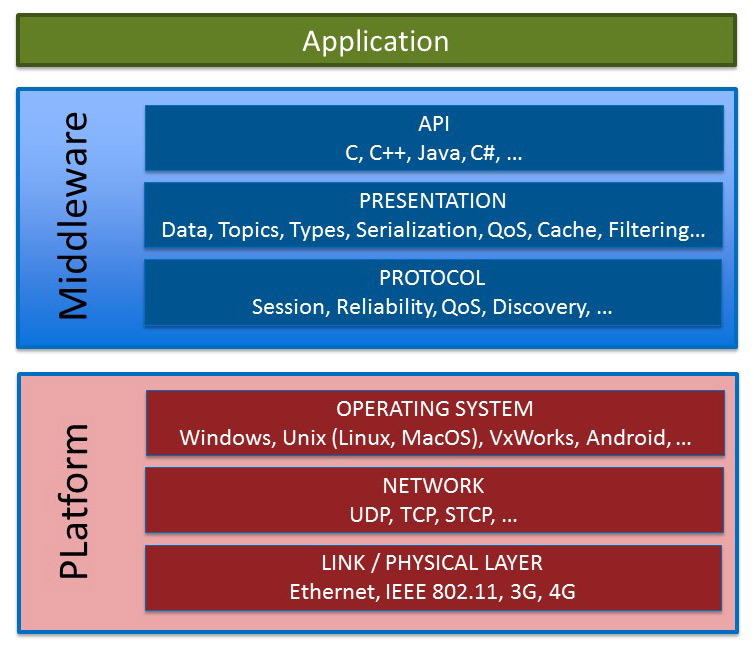
\includegraphics[scale=0.4]{fig/DDS.jpg}
\captionof{figure}[Software Layers in a Distributed System]{Software Layers in a Distributed System \cite{DDS}}
\label{fig:DDS}
\end{center}

\vspace*{0.5cm}
	
	{\bfseries Quality of Service (QoS)\nomenclature{QoS}{Quality of Service}}
	
	
	\vspace*{0.5cm}
	"The data can also be shared with flexible QoS specifications including reliability, system health (liveliness), and even security. DDS is smart about sending just what it needs. If messages don’t always reach their intended destinations, the middleware implements reliability where needed. When systems change, the middleware dynamically figures out where to send which data, and intelligently informs participants of the changes. If the total data size is huge, DDS intelligently filters and sends only the data each end-point really needs. When updates need to be fast, DDS sends multicast messages to update many remote applications at once. As data formats evolve, DDS keeps track of the versions used by various parts of the system and automatically translates. For security-critical applications, DDS controls access, enforces data flow paths, and encrypts data on-the-fly." \cite{DDS}
	
\vspace*{0.25cm}
	
The base QoS profile currently includes settings for the following policies:
\begin{itemize}

\item {\bfseries History}
\begin{itemize}
\item Keep last: This option only stores up to N samples, configurable via the queue depth option.

\item Keep all: This option stores all samples, subject to the configured resource limits of the underlying middleware.
\end{itemize}
\item {\bfseries Depth}
\begin{itemize}
\item Size of the queue: It is used to define N value when used together with keep last.
\end{itemize}
\item {\bfseries Reliability}
\begin{itemize}
\item Best effort: There is an attempt to deliver samples, but if the network is not robust, samples are lost.

\item Reliable: There is a guarantee that samples are delivered as the DDS may retry sending samples multiple times.
\end{itemize}
\item {\bfseries Durability}
\begin{itemize}
\item Transient local: The publisher becomes responsible for sending samples to late-joining subscribers.

\item Volatile: No attempt is made to persist sending samples.\cite{qos}
\end{itemize}
\end{itemize}

ROS 2, by default, has QoS set to reliable, keep last history, and volatile durability. In this thesis, only default QoS settings have been used as ROS 2 Crystal package was installed as a binary package which can be readily used. The user can only modify these settings through configuration files of DDS middleware and then installing ROS 2 packages by source. ROS 2 Dashing provides an easier way of changing QoS settings in the source code of the application via Node Options package.



	\section{Comparison of ROS 1 and ROS 2}	
	
	\vspace*{0.5cm}
In this section, major differences between ROS 1 and ROS 2 software architectures are stated with respect to the different layers. As described in the DDS section, the user does not need to know the underlying DDS schemantics in ROS 2 whereas in ROS 1, there is a master client to estabilish communication between nodes and the user has to know the custom transport and serialization packages to create an application. 


The major differences according to different software layers are:

\begin{itemize}
\item {\bfseries Application Layer}


\vspace*{0.25cm}
ROS 2 moves towards a distributed discovery mechanism where nodes advertise information to other nodes. ROS 1 has a centralized discovery mechanism where a master node is required to establish communication between nodes.
\vspace*{0.25cm}
\item {\bfseries Middleware Layer}


\vspace*{0.25cm}
ROS 2 uses DDS standard through which discovery, QoS policies, serialization, and transport is provided which also offers real-time support. ROS 2 also requires new versions of client libraries like C++11 and C++14 and Python 3.5 at least. ROS 1 uses a custom transport protocol, centralized discovery, custom serialization format, and uses C++3 and Python 2 versions.
\vspace*{0.25cm}
\item {\bfseries OS Layer}


\vspace*{0.25cm}
ROS 2 is supported on Linux, Windows 10, macOS and offers the possibility to run it on a RTOS, whereas ROS 1 is only supported on Linux.
\vspace*{0.25cm}
\end{itemize}
A summary of this comparison with respect to software layers is shown in figure 2.3.
			\begin{figure}[ht]
\begin{center}
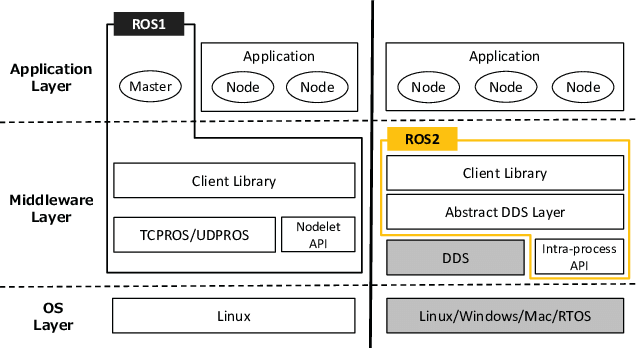
\includegraphics[scale=0.6]{fig/ros1_vs_ros2.jpg}
\caption[Comparison of ROS 1 and ROS 2 Architecture]{Comparison of ROS 1 and ROS 2 Architecture \cite{rosvsros2}}
\label{fig:rosvsros2}
\end{center}
\end{figure} 

With DDS as a standard middleware, the user can develop the application by using the standard application programming interfaces (APIs) defined by  ROS 2. \nomenclature{API}{Application Programming Interface}The user does not need to be aware of the underlying DDS APIs. The code can also be shared with other parties and can be modified or reused in similar use cases as it is built over a standard interface. ROS 2 supports new versions of client libraries which can be exploited for regularly updated APIs, the old APIs may lose support from their developers when the developers themselves switch to newer versions. Also, DDS supports real-time and embedded applications. A standardized system and support for other OSs leads to more number of users, variety of use cases and community contributed software improvement through issue reporting to ROS and its API developers.
	\section{Micro-ROS Architecture}
	\vspace*{0.5cm}
This section describes the micro-ROS architecture and explains how it enables support for embedded boards and real-time applications. Real-time applications also require a logical and pre-defined prioritization of tasks to be predictable, the execution strategy for this software has been explained in detail.
		\vspace*{0.5cm}

 
 
 {\bfseries Firmware/Client}
 
 
 \vspace*{0.5cm}
 The client is the microcontroller for which the micro-ROS software is cross-compiled (software is compiled on a different system than the target system) on the host - Linux and flashed onto the target - embedded microcontroller. All micro-ROS APIs are not needed on the board, they are only needed during compilation. The part of micro-ROS software (core libraries) flashed onto the target is called the firmware. The firmware uses Nuttx RTOS by default as its operating system. Nuttx can be configured to run different communication protocols and to run micro-ROS applications. Nuttx has a small footprint and is governed by the standards POSIX (Portable Operating System Interface)\nomenclature{POSIX}{Portable Operating System Interface} and ANSI (American National Standards Institute)\nomenclature{ANSI}{American National Standards Institute}. After enabling micro-ROS and related communication settings in the Nuttx configuration, the user can run the micro-ROS nodes on the microcontroller which can be accessed by Linux through Universal Serial Bus (USB)\nomenclature{USB}{Universal Serial Bus}. The firmware communicates with the host through the DDS-XRCE and connects to the agent running on the host.
 \vspace*{0.5cm}
 
 {\bfseries Agent/Server}
 
 
 \vspace*{0.5cm}
 The agent acts as a server for the clients and communicates with the microcontrollers. It runs on Linux and then can be used to connect with other ROS 2 nodes using the base ROS 2 versions.
 
  \vspace*{0.5cm}
Micro-ROS architecture is shown in figure 2.4. On the client side, core libraries of micro-ROS are flashed and the user can develop applications using core APIs. The  firmware uses Nuttx RTOS. The data exchange between client and server takes place by using DDS-XRCE. The server runs the micro-ROS Agent API which opens up the communication channel for an automatic discovery mechanism to connect with other ROS 2 nodes.
  \begin{center}
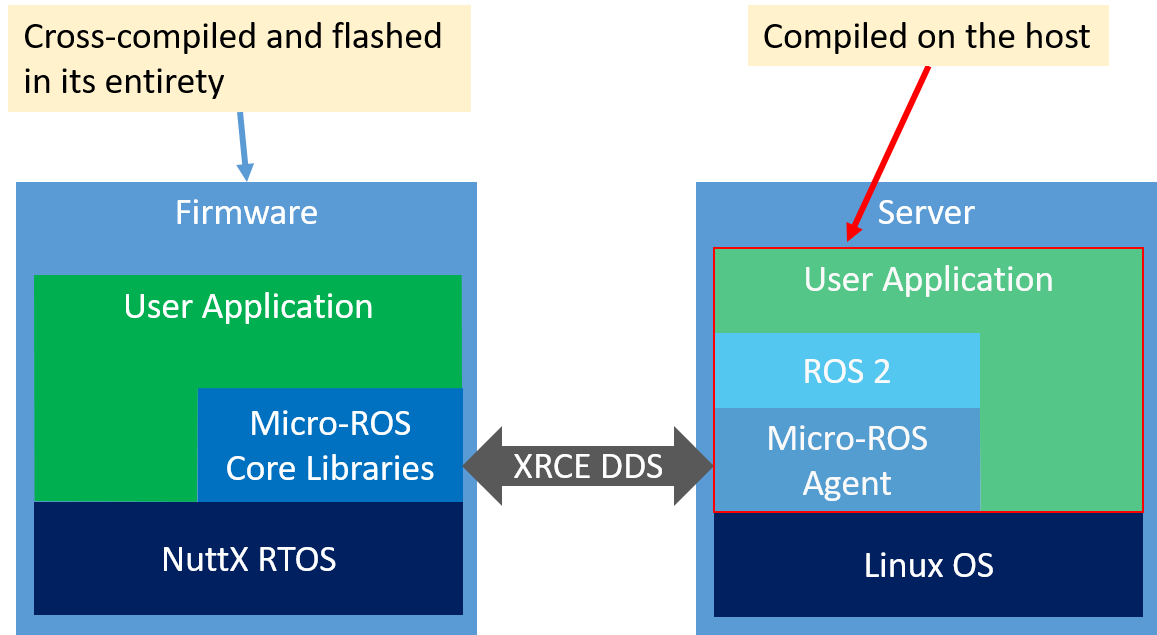
\includegraphics[scale=0.4]{fig/uros_arc.jpg}
\captionof{figure}[micro-ROS Architecture]{micro-ROS Architecture \cite{urosarc}}
\label{fig:urosarc}
\end{center}

  {\bfseries Real-Time Executor}
  \vspace*{0.5cm}
  
  
Robot applications require deterministic (predictable) execution of callbacks under all conditions and time constraints. Callbacks define the tasks which are to be performed in the node and they are called according to an update time or loop time. For example, callbacks in a node can subscribe to the laser scanner data, calculate the minimum distance to the object in front, and publish the command for the vehicle to stop when the distance is less than a specified value. Since the messages are buffered (pre-loaded in memory and ready for publishing or processing or subscription) in DDS, ROS 2 introduces the concept of executor, to support execution management (prioritization of callbacks). The standard ROS 2 executor does not have a pre-defined logic for executing a callback and also defines only one executor per process. It executes tasks based on the availability of entities (e.g. - publishers, subscribers, and messages). This is an error-prone approach as the software does not recognize which task is to be prioritized. For the above example, it may send the publisher data when the resources (e.g. - memory, processor, and executor) are available. This data might not be useful to the user when the input laser data changes and reaches the specified value of minimum distance to the object. Brake command is expected from the publisher but it may arrive too late and can result in an accident. Therefore, deterministic execution of callbacks under time constraints cannot be guaranteed.


"The Logical Execution Time (LET)\nomenclature{LET}{Logical Execution Time} is a known concept in automotive domain to simplify synchronization in process scheduling. It refers to the concept to schedule multiple ready tasks in such a way, that first all input data is read for all tasks, and then all tasks are executed."\cite{let}

First, a static scheduling order is defined. For example, after defining a subscription callback, a publisher callback, and a ROS node, then a subscriber object and a publisher object are defined. The executor is initialized with these two objects and then a function in the executor is used to define the scheduling order of the subscription callback before the publisher callback. The user can define some computation of the subscriber object and use it for the publisher object or create a condition for the publisher, using the subscriber object. Therefore, the subscriber object will always be processed before the publisher object. Finally, the executor is allowed to run which is continuously called as per the default loop time or custom loop time set by the user.

This 2 step approach of the LET Executor guarantees a deterministic execution of callbacks.
 
	\section{Used Hardware and Communication Protocols}
	\vspace*{0.5cm}
In this section, embedded hardware systems and communication protocols used with ROS 2 in this thesis work are described in brief. 	
	\vspace*{0.5cm}
	
	{\bfseries STM32 Microcontroller}
	
	
	\vspace*{0.5cm}
A Microcontroller Unit (MCU)\nomenclature{MCU}{Microcontroller Unit} is a compact, integrated circuit which includes input/output peripherals, memory and a processor on a single chip. It is designed to govern a specific operation and is commonly found in automobiles, robots, mobile devices, and vending machines. In this thesis work, 32-bit MCUs have been used from the STM family of microcontroller boards. Two development boards, see figure 2.5, Olimex STM32-E407 and Waveshare STM32-Open407I-C, having similar architectures have been used for testing.

\begin{center}
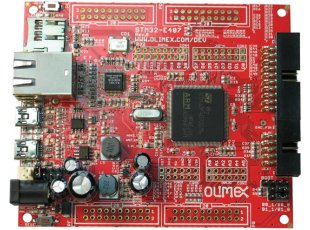
\includegraphics[scale=0.55]{fig/STM32-E407.jpg}\hspace*{1cm}
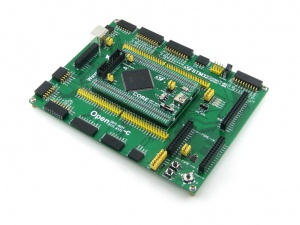
\includegraphics[scale=0.65]{fig/Open407I-C.jpg}


\captionof{figure}[Olimex-STM32-E407 and Waveshare STM32-Open407I-C]{Olimex-STM32-E407 (left) \cite{olimex} and Waveshare STM32-Open407I-C (right) \cite{waveshare}}
\label{fig:stm32}
\end{center}
\vspace*{0.5cm}	

{\bfseries Communication Protocols}
	
	
\vspace*{0.5cm}
The communication protocols used in testing of micro-ROS are:
\begin{itemize}
\item {\bfseries Internet Protocol (IP)}\nomenclature{IP}{Internet Protocol} - It is the main communication protocol to transmit datagrams across network boundaries through IP addresses. The MCU is assigned an IP address and a local area network is setup through ethernet wires between the computer and the MCUs to enable the micro-ROS client-agent connection. User Datagram Protocol (UDP),\nomenclature{UDP}{User Datagram Protocol} part of IP suite, supported by micro-ROS is used in this thesis work.
\item {\bfseries USB-Serial} - PL2303 peripheral device is used to connect the board’s UART (Universal Asynchronous Receiver-Transmitter)\nomenclature{UART}{Universal Asynchronous Receiver-Transmitter} pins to the USB of the computer to enable communication via USB wire. However, the speed of data transfer is slower than IP because of the PL2303 driver used.
\item {\bfseries Inter-Integrated Circuit (I2C)}\nomenclature{I2C}{Inter-Integrated Circuit} - It is a multi-wire serial bus protocol to allow communication between small chips (slaves) with bigger chips (master). In this thesis work, a demonstrator for micro-ROS using a digital air pressure sensor was built which uses I2C protocol between the sensor and the MCU.
\end{itemize}

	
	\section{Real-Time Systems}
	
	
	\vspace*{0.5cm}	
Real-time systems should produce reproducible and correct computations at the correct time and be predictable even in worst-case scenario. Failure to respond within a set desired time (deadline) can cause damage to life or other resources. These systems have to be designed according to the dynamics of the physical process. They are often part of an embedded system and are employed in airplane systems, automotive systems, satellites, power stations, and other critical applications. These systems are usually resource-constrained but still should offer low latencies. Latency is the delay in transfer of data after the data transfer is requested. Jitter is the variation in the periodic loop time.
	
	
Figure 2.6 shows desired time, jitter with reference to the loop time. Overrun is the instance when the time exceeds the acceptable jitter value.
	\begin{center}
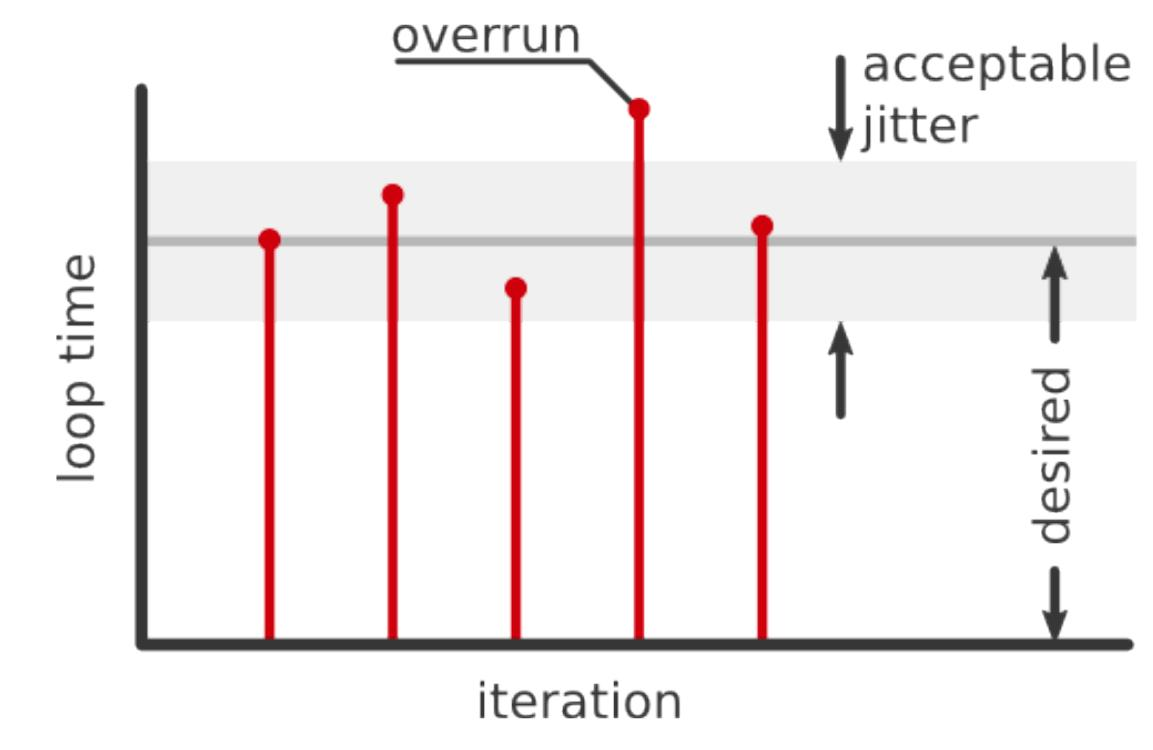
\includegraphics[scale=0.5]{fig/deadline.jpg}
\captionof{figure}[Deadline and Jitter in Real-Time Systems]{Deadline and Jitter in Real-Time Systems \cite{deadline}}
\label{fig:deadline}
\end{center}
	The different types of real-time systems are:
	\begin{itemize}
\item	{\bfseries Soft} - The result can still be used after the deadline. For example, audio/video playback failure will only cause irritation to the user.
\item	{\bfseries	Firm} - The result does not have utility after the deadline. For example, in an automated manufacturing facility with high production rate, if the part does not arrive in time for a process to take place and the part is skipped or the machines stop, then it can cause financial losses to the facility.
\item	{\bfseries	Hard} - Missing a deadline can be catastrophic and can cause serious damage to life and property. For example, the landing gear of an airplane fails to deploy in time during an emergency landing.
	\end{itemize}
	\clearpage
	
	\section{Available Research on Real-Time Testing of ROS 2}
\vspace*{0.5cm}
ROS 2 developers (Open Robotics), Bosch, and Nobleo Technology have already tested some aspects of the real-time performance of ROS 2. Their results and challenges related to real-time performance are stated as follows: 
\begin{itemize}
\item {\bfseries Inverted pendulum demo results} - The unstable arrangement of an inverted-pendulum is used as a means to test the real-time performance of ROS 2. A simulation is performed with ROS 2 where the pendulum is balanced by a motor and a moving cart at the base. The motor command and sensor feedback are configured as ROS 2 messages and these are updated with a loop time of 1 ms. Linux preemptible kernel is used which offers real-time capability. High scheduling priority is given to the node and memory allocations are done during initialization of the node. Dynamic memory allocations are blocked as they are not real-time safe. J. Kay and A.R. Tsouroukdissian have implemented this package with ROS 2 Alpha release. They also mentioned that DDS can be fine-tuned for better real-time performance. Their goal was to get less than 3 \% (30 \si\micro s) jitter. Without any stress to the system, the maximum jitter was 3.51 \%, minimum was 0.16 \%, and mean was 0.46 \% but with stress on the processor, the maximum jitter was 25.8 \%, minimum was 0.14 \%, and mean was 0.38 \%. Also, 3 instances of overrun were observed.


Figure 2.7 describes the inverted pendulum setup and how the real-time process is separated from non real-time processes. The computational processes are real-time tasks and logging of data or user command to disturb the setup during run time are non real-time tasks.
	\begin{center}
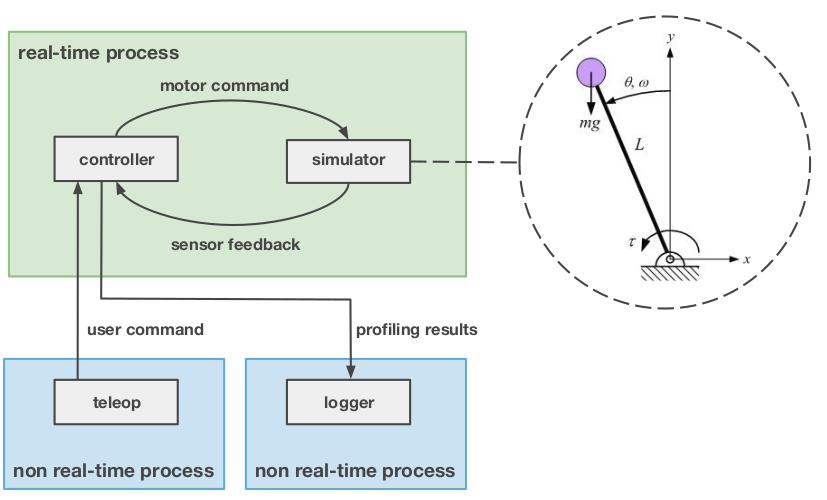
\includegraphics[scale=0.6]{fig/inverted.jpg}

\captionof{figure}[Inverted Pendulum Setup]{Inverted Pendulum Setup \cite{deadline}}
\label{fig:inverpen}
\end{center}
\item {\bfseries Non-deterministic scheduling by ROS 2 standard executor} - In a recent study by researchers at Bosch (for more details, see \cite{ingo}), it has been found that the ROS 2 C++ Executor in version Crystal Clemmys has some undesired properties for real-time scheduling. They are:
\begin{itemize}
\item The Executor gives highest priority to timers and therefore messages from the DDS queue are not processed in overloaded situations. Timers are used to schedule a callback at a specific rate or update time independent to the executor time. They do not define the scheduling order and cannot be used for scheduling real-time tasks.
\item Non-preemptive round-robin scheduling of non-timer handles/entities (subscriptions, services,clients) leads to priority inversion, lower priority callbacks may block higher priority callbacks leading to high processing time. Also, this problem is further aggravated as only one message per handle is considered, even when multiple messages of the same topic are available, only one instance is processed by the executor which causes backlog and hence, priority inversion. 
\end{itemize} 
These shortcomings led to the development of the LET Executor in micro-ROS to allow for deterministic execution.
\item {\bfseries High CPU Overhead by ROS 2 Executor} - In a study by Nobleo Technology (see \cite{nobleo}), it has been concluded that the ROS 2 SingleThreadedExecutor uses 70 \% CPU power and generates CPU overhead (e.g. - unnecessary computation or memory allocations). ROS 2 Executor needs to be optimized otherwise normal ROS 2 cannot function properly on ARM Cortex-A class embedded boards. Cortex-A class chips are 32-bit and 64-bit microprocessors or chips licensed by ARM. Nobleo also presented an alternative static executor to reduce overhead but it has still not been approved for the next ROS 2 release.
\end{itemize}


	\chapter{ADAS Applications using ROS 2}
		
\rofoot[\pagemark]{\pagemark}
\refoot[\pagemark]{\pagemark}
This is an open-source project using License Apache 2.0 to understand simple ADAS applications using ROS 2 Crystal and the Gazebo simulator. The user can drive around the robot in the simulator and have lane detection and automatic braking when an object is detected. To run this simulator, please refer to the instructions given in the Github repository, see - \href{https://github.com/Viplav04/ADAS-ROS2-Gazebo-Simulator}{"ADAS Simulator using ROS 2 and Gazebo"} \cite{ADASsim}.
ROS 2 and Gazebo are both developed by Open Robotics. There are various plugins available to convert Gazebo data to ROS 2 data. A camera sensor and a laser sensor have been used in the simulator with a robot which also has a differential drive and can be driven around with the help of a keyboard. The algorithms were developed using C++ language.

Figure 3.1 shows the communication connections of the simulator through plugins with ROS 2 nodes. The user has access to a keyboard and lane detection output from the camera. 

	\begin{center}
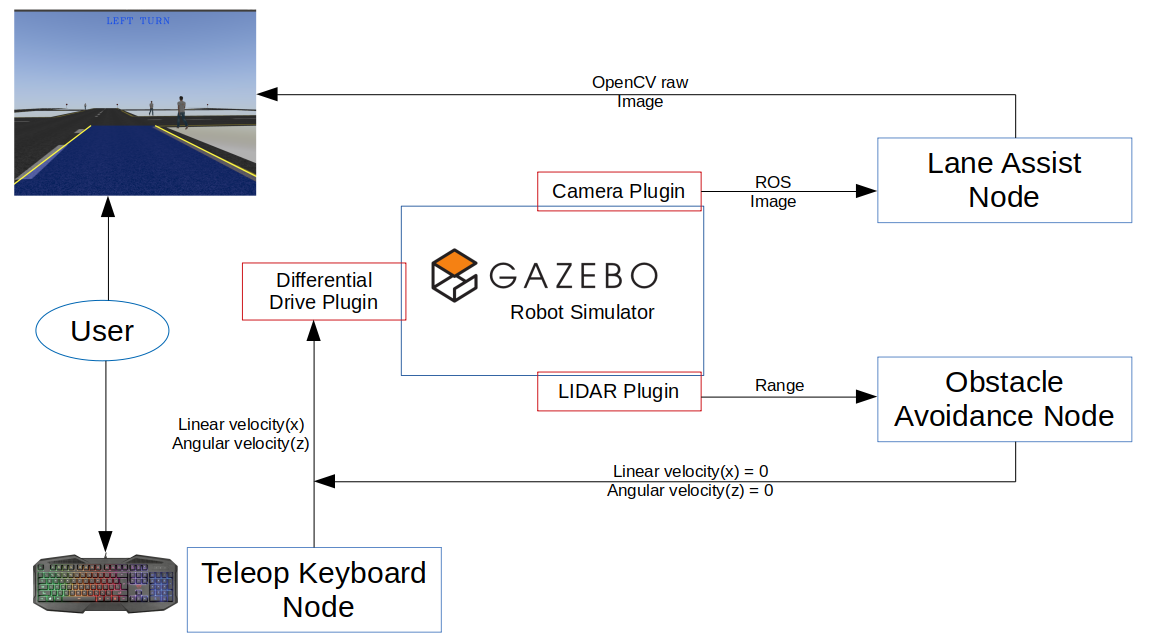
\includegraphics[scale=0.4]{fig/ros2adas.png}
\captionof{figure}[ADAS Simulator using ROS 2 and Gazebo]{ADAS Simulator using ROS 2 and Gazebo}
\label{fig:ADAS}

\end{center}


First, a "customworld.world" file is created in the Gazebo simulator and then, roads and humans are added to the world. The robot is modified from the differential drive demo already available in ROS 2 Gazebo tutorials and a camera and laser sensor is then attached to it. This setup consists of 3 nodes as explained in the next sections.
		\section{Camera Lane Detection}
	\vspace*{0.5cm}
	Important steps to do lane detection for an image are : 
	\begin{enumerate}
\item	The input image subscribed from Gazebo simulator is a ROS message, output from the camera plugin. First, it has to be encoded to a raw image to use Open Computer Vision (OpenCV)\nomenclature{OpenCV}{Open Computer Vision} libraries. The raw image is then converted to a grayscale image. Figure 3.2 shows the robot in the Gazebo world. 
\begin{center}
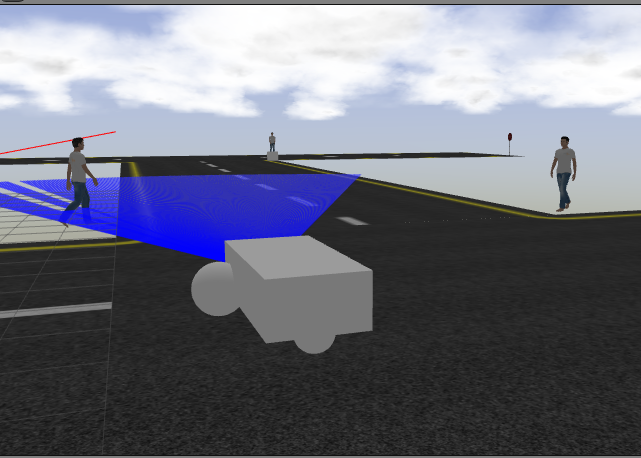
\includegraphics[scale=0.4]{fig/canny1.png}
\captionof{figure}[Gazebo Environment]{Gazebo Environment}
\label{fig:gazebo}
\end{center}
\item Canny Edge Detector from OpenCV libraries is applied to the greyscale image to detect edges as shown in figure 3.3.
	\begin{center}
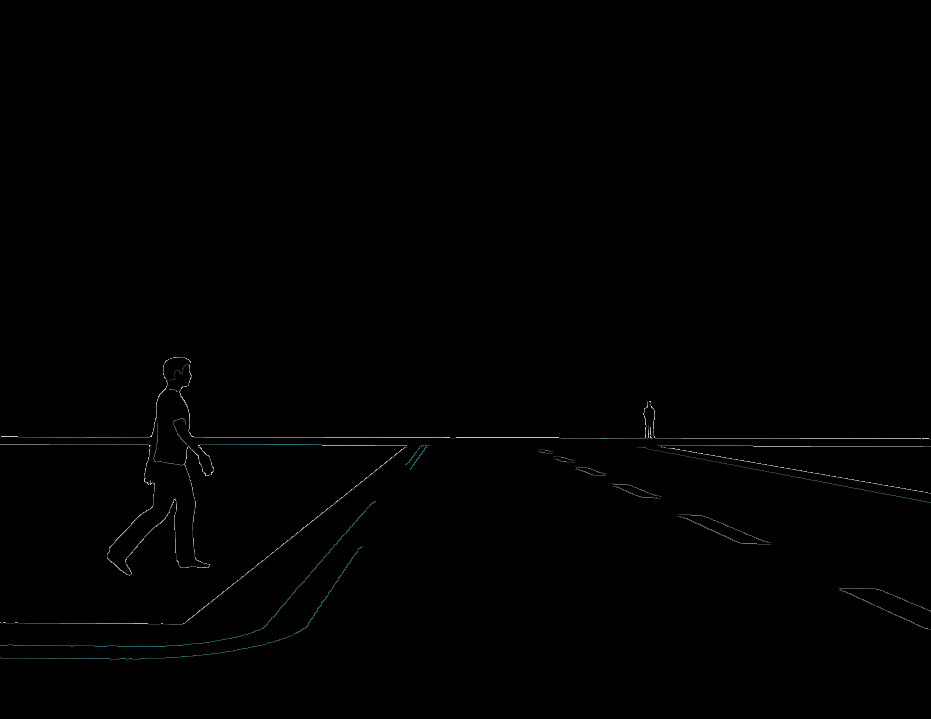
\includegraphics[scale=0.3]{fig/canny.png}
\captionof{figure}[Canny Edge Detection]{Canny Edge Detection}
\label{fig:canny}
\end{center}
\item An image mask is created according to the input image size which filters out the edges in the bottom half of the screen to show only the bottom edges. Then, Hough Transform function from OpenCV libraries is applied to the resulting image which detects straight lines. The straight lines are then superimposed to the original raw image as shown in figure 3.4.
\begin{center}
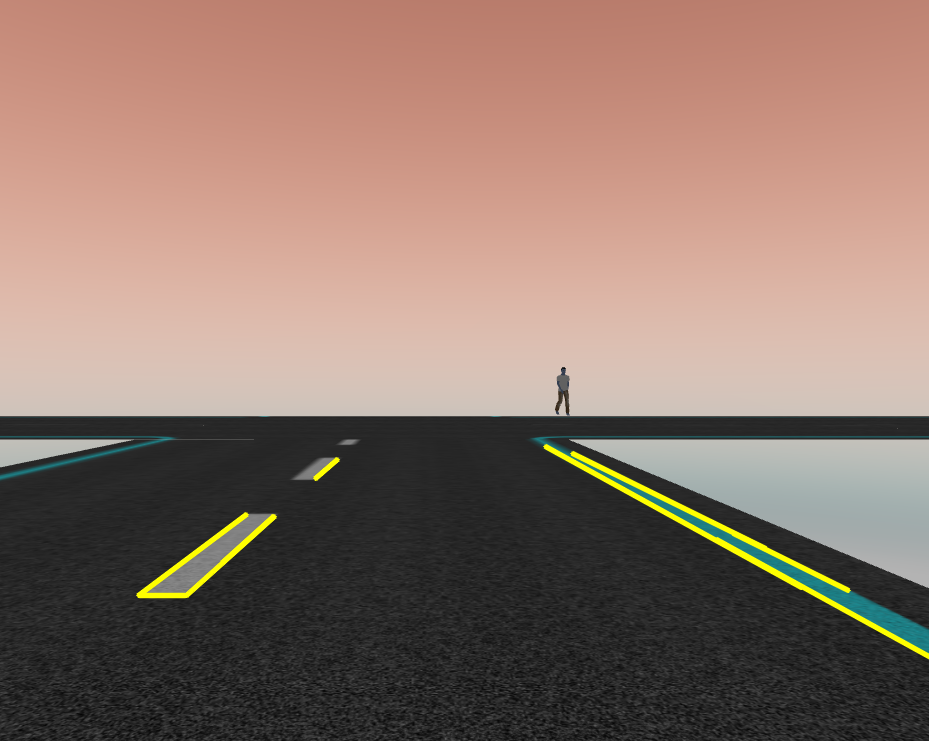
\includegraphics[scale=0.3]{fig/hough.png}
\captionof{figure}[Line Detection using Hough Transform]{Line Detection using Hough Transform}
\label{fig:hough}
\end{center}
\item The lines detected are further optimized and a box is drawn connecting the two lines to display the lane. Also, as shown in figure 3.5, turning advice to stay in the lane is printed onto the image calculating the direction in which the robot is heading.
\begin{center}
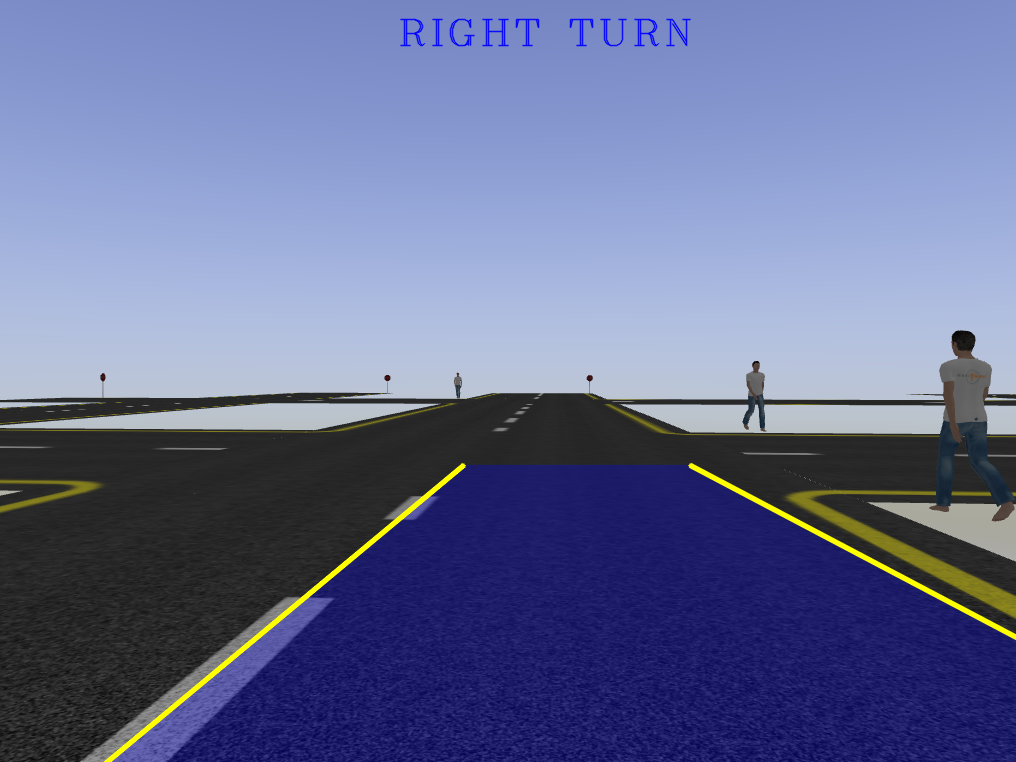
\includegraphics[scale=0.3]{fig/finaladas.png}
\captionof{figure}[Lane Detection]{Lane Detection}
\label{fig:lane}
\end{center}
	\end{enumerate}
		
				\section{Driver Control by Keyboard}	
	\vspace*{0.25cm}
The robot has 3 wheels and a differential drive to enable turning. ROS 2 offers a built-in "teleop\textunderscore twist\textunderscore keyboard" package to send messages to the robot from the keyboard. The messages are already available in ROS 2 known as "Twist" messages. The differential drive plugin with Gazebo simulator can be enabled by modifying the robot model file in Gazebo. The user can limit the maximum velocities (in this work - 2 m/s) of the robot with this package. 	

		\section{LIDAR based Auto Stop}
		\vspace*{0.25cm}
		
The laser sensor data gives out the minimum range of any object in its field. Range messages are already available in ROS 2. Then, an algorithm is applied to the incoming data and a condition is added. When the object is within a range of 4 m, this node publishes a new "Twist" message to the robot telling it to stop. Also, it sends a "STOP, Reverse or Change direction" comment to the user in the Linux terminal and also prints it out in the image running in the lane detection node. The laser data can be visualized in the RViz package of ROS 2 as shown in figure 3.6. The user can observe the point cloud (set of points which show the external surfaces of the objects) and can use this data for further computation.
			\begin{center}
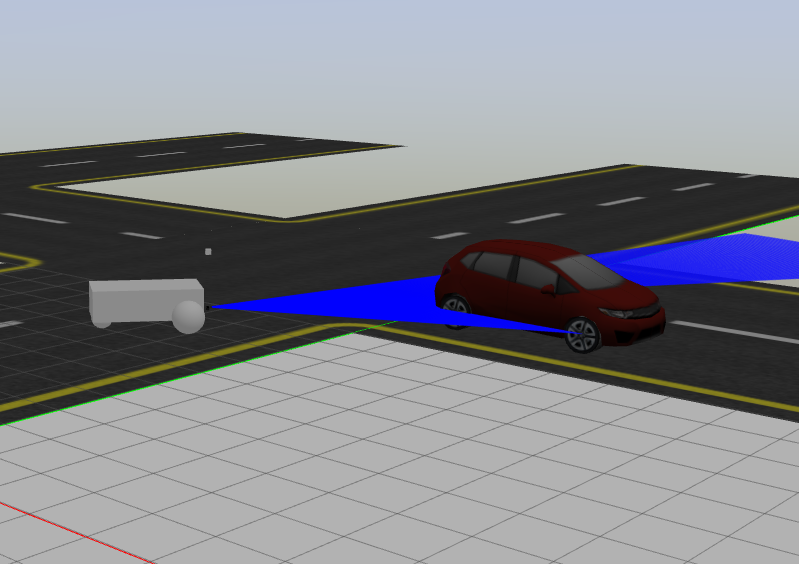
\includegraphics[scale=0.3]{fig/laser.png}
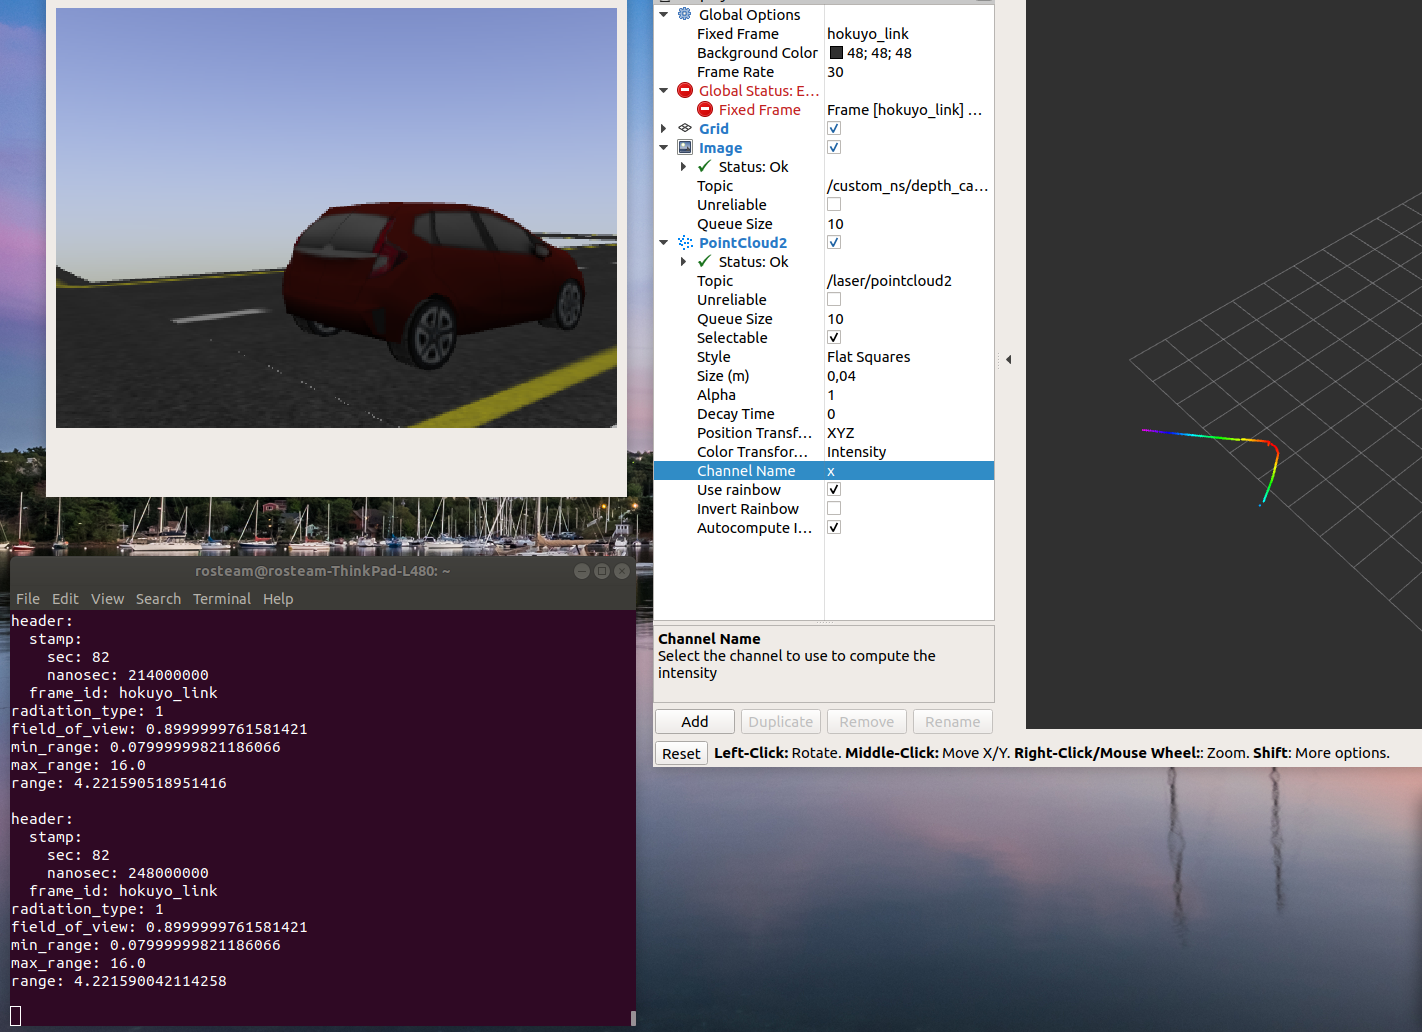
\includegraphics[scale=0.17]{fig/laser2.png}
\captionof{figure}[Laser and Camera Data Visualization]{Laser and Camera Data Visualization}
\label{fig:laser}
\end{center}

Figure 3.7 shows the Auto Stop feature when a human is within the minimum range and stops the robot.
			\begin{center}
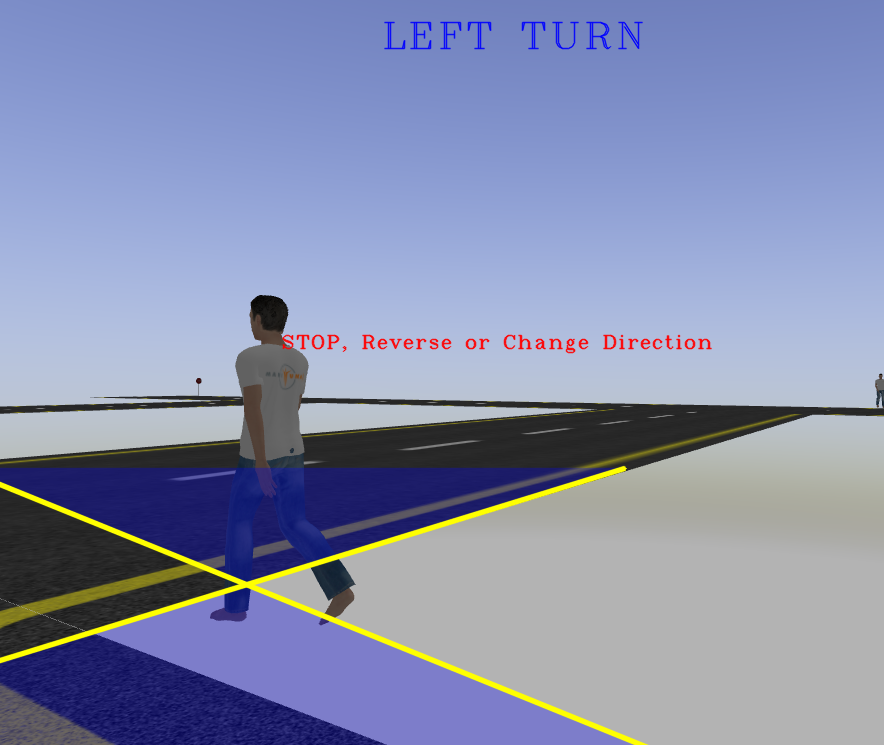
\includegraphics[scale=0.3]{fig/final2adas.png}
\captionof{figure}[Auto Stop Feature]{Auto Stop Feature}
\label{fig:lane1}
\end{center}
This project helps in understanding ROS 2 concepts and also explore its versatile libraries. Along with the Gazebo simulator, different kinds of robot applications can be tested and simulated for worst-case scenarios, especially for ADAS systems and automated driving applications where physical testing of systems requires significant resources. 

Different types of data can be accessed in a single node with multiple publishers or subscribers. Also, nodes can interact and discover themselves automatically, the user just has to source the ROS 2 software and launch the created nodes in different terminals in Linux.
	\chapter{Test Setup}
		
\rofoot[\pagemark]{\pagemark}
\refoot[\pagemark]{\pagemark}
The main part of this thesis work was to set up the micro-ROS environment on the STM32 Embedded board and test it, but ROS 2 testing packages were also available and therefore the standard ROS 2 stack was also tested. The procedure to setup the test environments for both ROS 2 and micro-ROS have been described in this chapter.
	
\section{Test Application for ROS 2}
\vspace*{0.5cm}
The testing of ROS 2 is based on the inverted pendulum demo. The demo is different for ROS 2 Crystal and Dashing versions. ROS 2 Crystal has an in-built demo as part of its packages. There is another version of this demo in development for ROS 2 Dashing and newer versions. We can also visualize the inverted pendulum simulation in RViz for the Dashing version as shown in figure 4.1. The blue inverted pendulum tends to fall down but the red cart tries to balance it. Real-time performance can be tested by these packages as they are based on the concept of node lifecycle which seperates the real-time processes from the non real-time tasks.
			\begin{center}
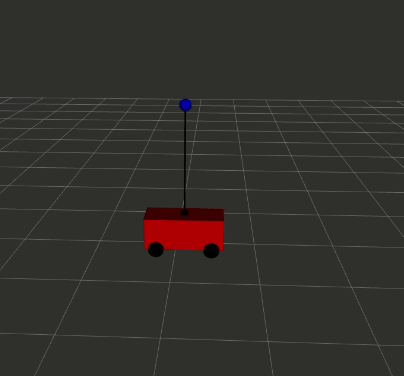
\includegraphics[scale=0.51]{fig/invertedpendulum.png}
\captionof{figure}[Inverted Pendulum Simulation in RViz]{Inverted Pendulum Simulation in RViz}
\label{fig:invertedpendulum}
\end{center}

	\subsection{Components}
	\vspace*{0.5cm}
Hardware and software components required to perform this testing were:
	\begin{itemize}
	\item A Linux system with Ubuntu 18.04 installed.
	\item Linux real-time patch was applied after installing RT-PREEMPT kernel which offers real-time testing capability.
	\item ROS 2 Crystal and Dashing versions were installed.
	\item Inverted Pendulum demo for Dashing is required. It can be downloaded from - \href{https://github.com/ros2-realtime-demo/pendulum}{"ROS2-realtime-demo"} \cite{rtpendulum}.
	\end{itemize}
	\subsection{Procedure}	
\vspace*{0.5cm}
The user needs to set real-time settings in Linux and build the Dashing pendulum demo environment. The steps to set up the environment and run the demo for both Crystal and Dashing are explained in this section. 
\vspace*{0.25cm}


{\bfseries To set real-time settings in Linux kernel}:
\begin{itemize}
\item Ubuntu 18.04 has a security feature called "SecureBoot" to not allow unsigned kernels to be booted. Therefore, the real-time (RT-PREEMPT) kernel has to be signed after installation. To do this, see \href{https://askubuntu.com/questions/1081472/vmlinuz-4-18-12-041812-generic-has-invalid-signature}{"Signing a kernel"} \cite{dualboot}.
\item To set memory locking and high real-time scheduling priority, the following lines were added to the end of the file "/etc/security/limits.conf" :
\begin{itemize}
\item "<username>  - memlock limit-in-kilobytes(kB)". This limit was set to 1000 kB\nomenclature{kB}{Kilobyte} as per instructions by pendulum demo package developers.
\item "<username>  - rtprio 75". Warning: Never set priority to 99 as it may interfere with important computer processes.
\item The user has to logout and login again to see the changes. The user needs to run the demo as root, type "sudo su" in a terminal and enter the password to have access to real-time settings.
\end{itemize}
\end{itemize}

{\bfseries To run demo with ROS 2 Crystal}:
\begin{itemize}
\item The ROS 2 Crystal setup.bash file is sourced in a terminal (as root user) and "pendulum\textunderscore demo>output.txt" command is executed. The node writes the output to the text file.
\item This node sends a 1000 messages for both the motor controller and feedback sensor with an update rate of 1 ms. This process was repeated 5 times and the values were recorded.
\item Then in another terminal "stress --cpu 100" command was launched and also many applications were launched in the computer to put stress on the CPU and memory. Then, pendulum demo was launched 5 times and values were recorded.
\end{itemize}
{\bfseries To run demo with ROS 2 Dashing}:
\begin{itemize}
\item The pendulum demo package was downloaded in a "pendulum\textunderscore ws" folder and the environment is built. To run this demo, see instructions in Github repository - \href{https://github.com/ros2-realtime-demo/pendulum}{"ROS2-realtime-demo"} \cite{rtpendulum}. 1000 kB of memory is locked for this node.
\item This is a continuous simulation. In another terminal, after sourcing the ROS 2 Dashing environment and pendulum environment, "ros2 topic list" command is run. If the demo is enabled with "--pub-stats" as in the instructions, we should see controller and driver statistics topics. They can be launched by command "ros2 topic echo /topic\textunderscore name ". Then in another terminal, "stress --cpu 100" command was launched.
\item The values were recorded every minute and the simulation was allowed to run for 10 minutes.
\end{itemize}
\section{Testing of micro-ROS}
\vspace*{0.5cm}
This testing has been done with micro-ROS Crystal version. Dashing version is still not officially released and there were installation issues with it. The hardware required for this testing has been listed in the components sub-section. The steps to set-up the hardware are then described in the procedure sub-section.
	\subsection{Components}
	\vspace*{0.5cm}
Hardware and software components required for testing micro-ROS were:	
	\begin{itemize}
	\item A Linux OS with Ubuntu 18.04 and micro-ROS and Nuttx repositories installed.
	\item One Olimex STM32-E407 MCU.
	\item One Waveshare STM32-Open407I-C MCU.
	\item One USB to TTL UART PL-2303 converter cable.
	\item One Waveshare UART TTL to ethernet converter DP83848.
	\item Three ethernet cables.
	\item Four UART cables.
	\item One BMP180 pressure sensor.
	\item One Olimex JTAG USB OCD ARM debugger (ARM-USB-OCD-H).
	\item Two Micro-USB cables.
	\end{itemize}
	\subsection{Procedure}	
	\vspace*{0.5cm}
	The steps to perform this testing are enlisted below:
\begin{enumerate}
	\item Micro-ROS and Nuttx repositories were installed in "uros\textunderscore ws" folder by following the instructions in this link - \href{https://micro-ros.github.io/docs/tutorials/basic/getting_started/}{"micro-ROS Installation"} \cite{urosinstall}.
	\item In this setup, 2 boards with similar architectures were used. Waveshare board was made to work on a serial transport connection and the Olimex board with ethernet (UDP). 
	
There is a configuration file (.config) in directory -

"/uros\textunderscore ws/firmware/mcu\textunderscore ws/uros/rmw\textunderscore microxrcedds/rmw\textunderscore microxrcedds\textunderscore c/" where the type of transport and IP address can be changed.

	\item The next step was to configure Nuttx to work with micro-ROS, pressure sensor, USB console, ethernet, and debugging features. 
It was important to understand the configuration of the Nuttx RTOS. Videos from the \href{https://www.youtube.com/channel/UC0QciIlcUnjJkL5yJJBmluw/videos}{"Nuttx Channel"} \cite{Nuttxchannel} were referred to enable the required hardware and communication settings. The architecture and configuration of an OS is an exhaustive topic and cannot be explained in brief. But these videos have exact details to enable the pressure sensor, USB console, ethernet, debugging, and external applications like micro-ROS and "delay\textunderscore test". 
	
	A working configuration file can be found at this repository - \href{https://github.com/Viplav04/NuttX/tree/master/configs/olimex-stm32-e407/uros}{"micro-ROS Configuration File"} \cite{olimexconfigfile}.
	\item After configuring Nuttx, the firmware was flashed onto the board (see - \href{https://micro-ros.github.io/docs/tutorials/basic/getting_started/}{"micro-ROS Installation"} \cite{urosinstall}). JTAG debugger should be connected to the board for flashing. Micro-USB cable is used to access the board's operating system (console) at Linux. Figure 4.2 shows the connection of the JTAG debugger and micro-USB cable with the Olimex MCU. 
	
				\begin{center}
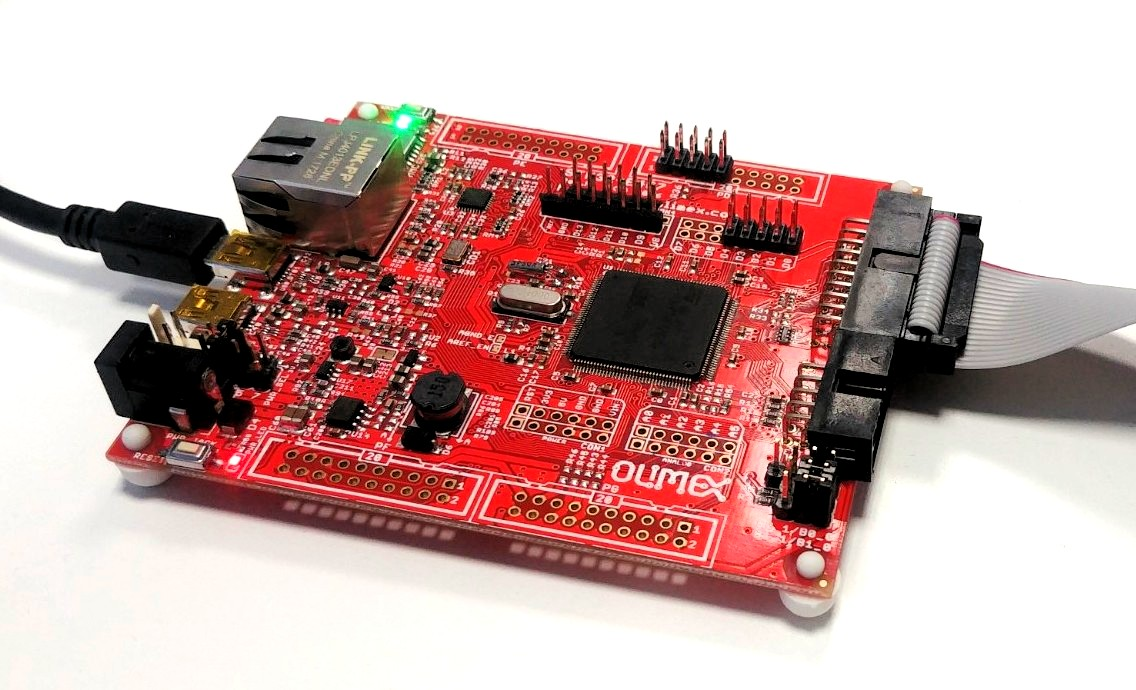
\includegraphics[scale=0.2]{fig/olimexnshusb.jpg}
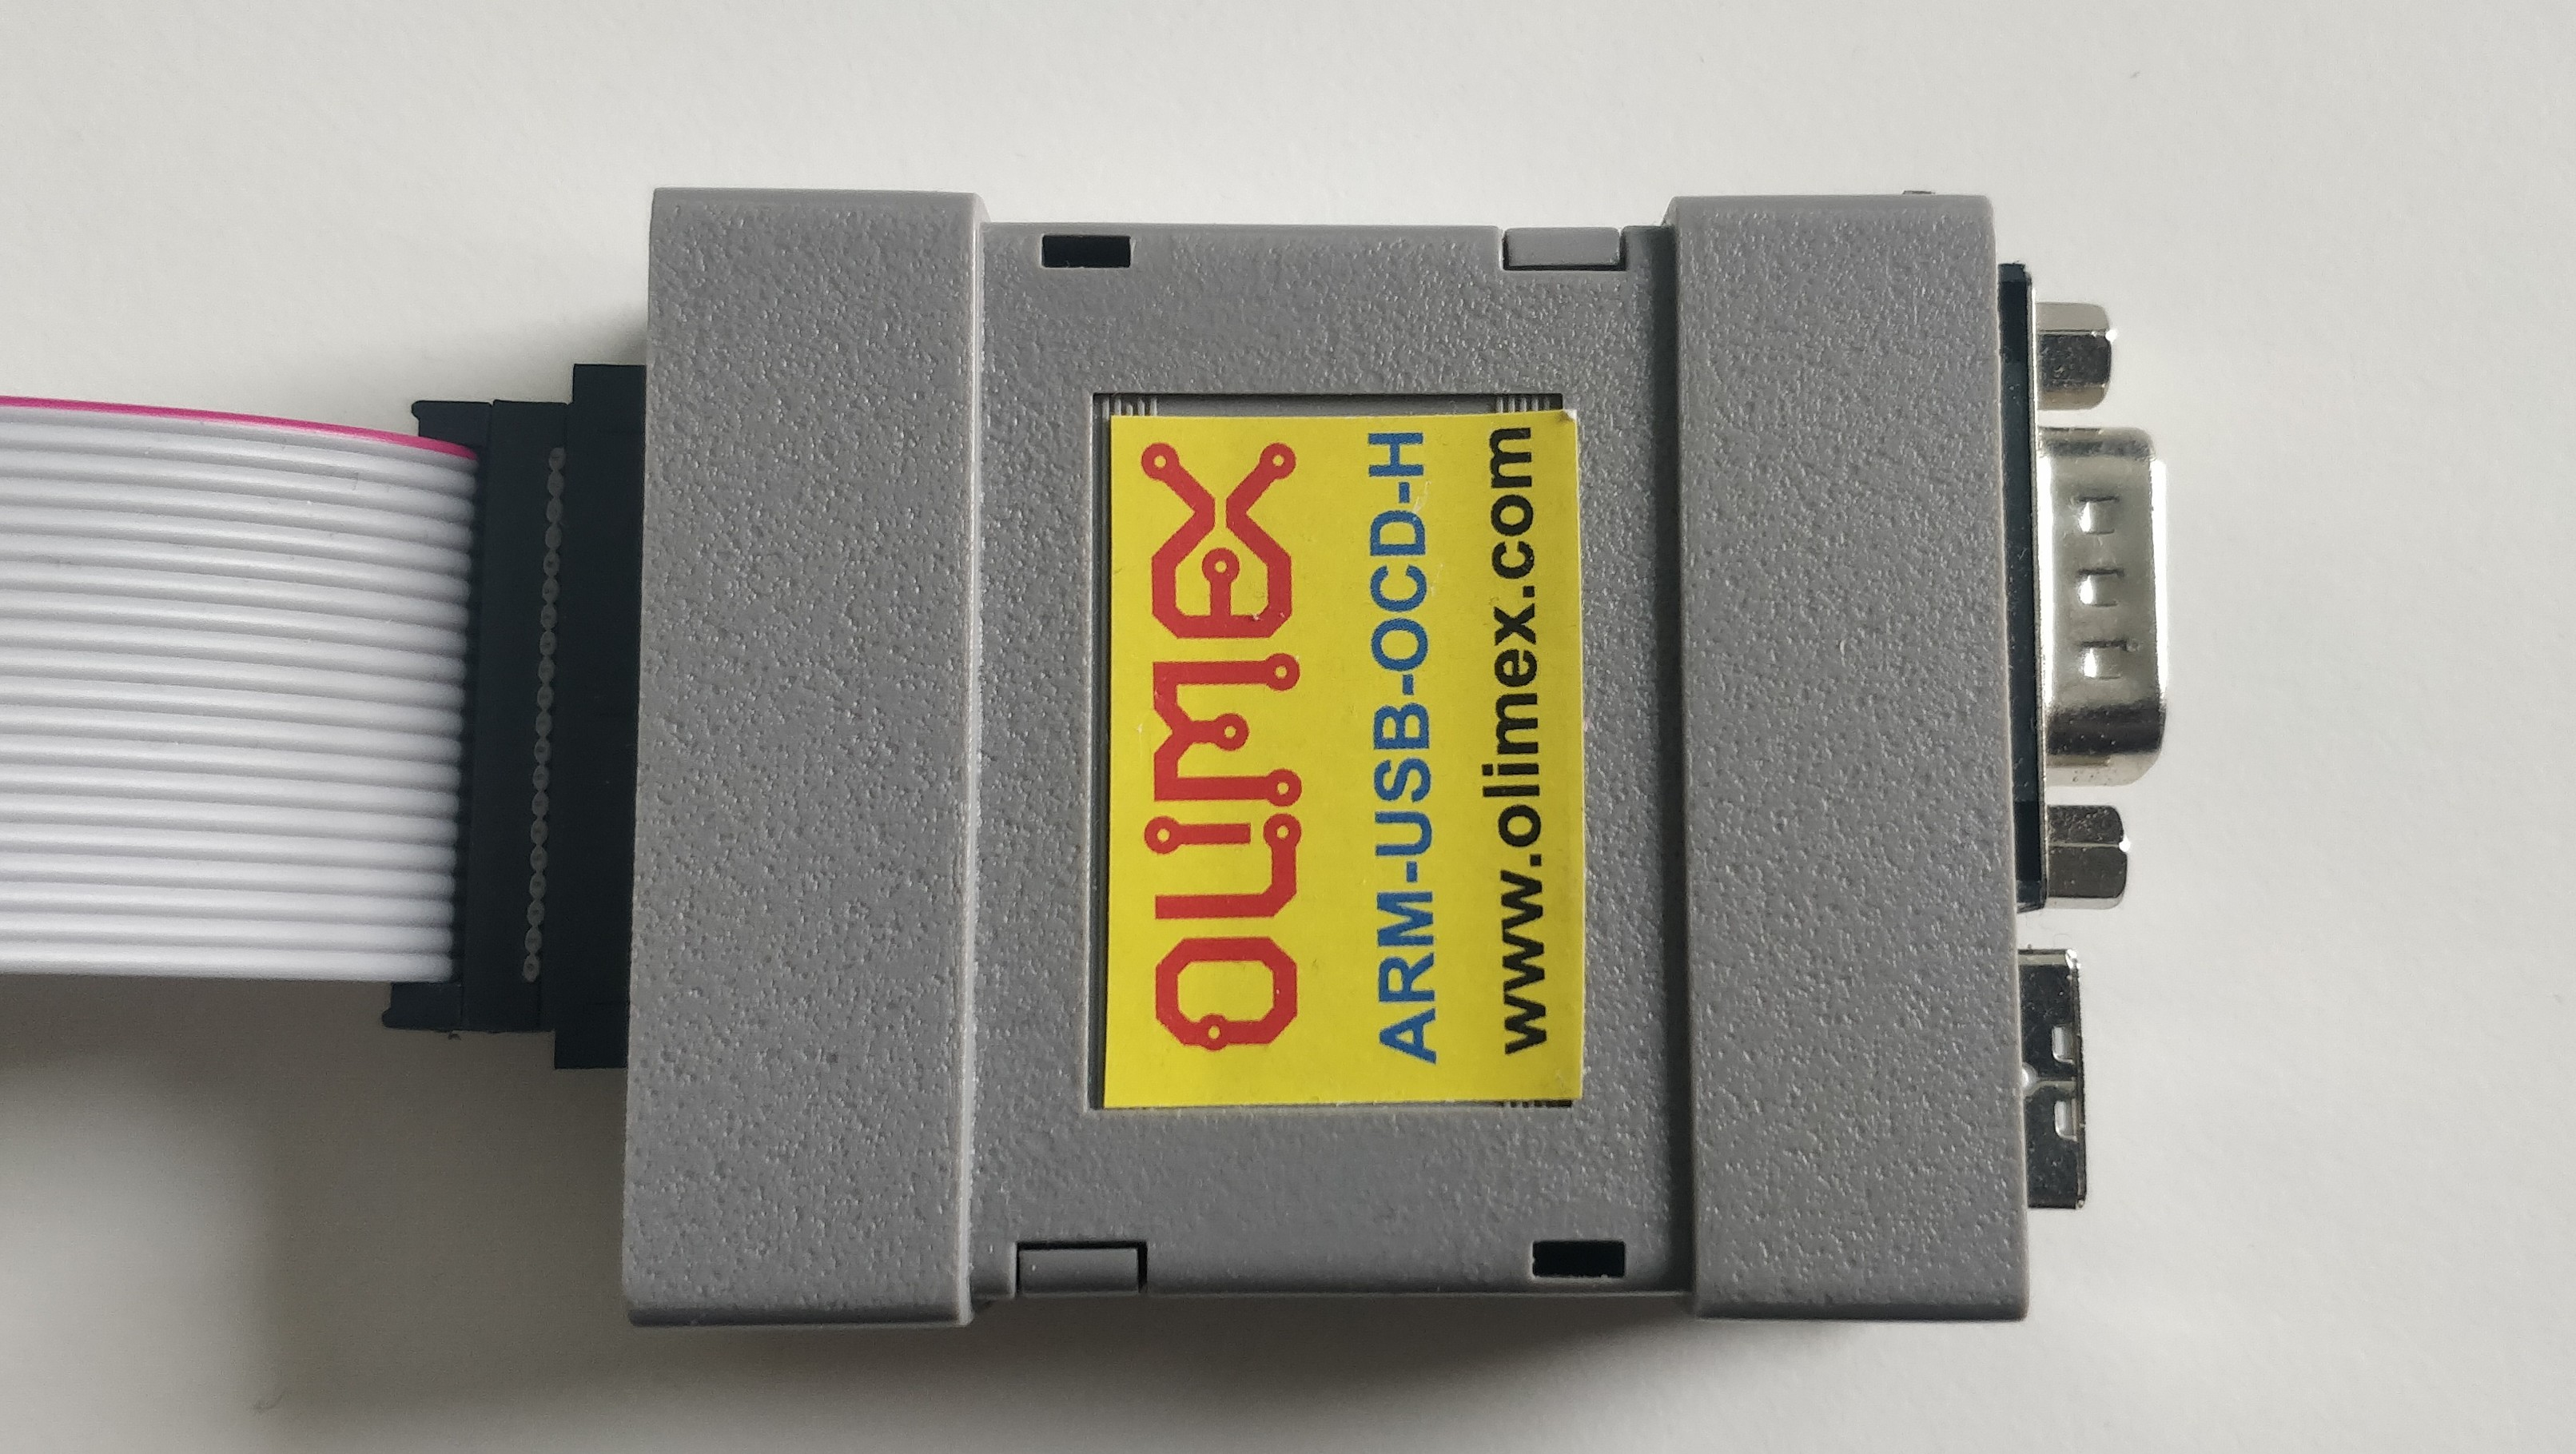
\includegraphics[scale=0.05]{fig/jtagusbocd.jpg}

\captionof{figure}[Olimex-STM32-E407 with JTAG Debugger]{Olimex-STM32-E407 with JTAG Debugger}
\label{fig:jtag}
\end{center}
\item To connect the pressure sensor with the board (board's datasheet is required, see - \href{https://www.olimex.com/Products/ARM/ST/STM32-E407/resources/STM32-E407.pdf}{"Olimex-stm32-e407 datasheet"} \cite{olimexdatasheet}), 4 UART cables are connected in the following sequence:

\begin{itemize}
\item Connect Vcc to board's 3V(volts) terminal.
\item Connect GND to board's Ground terminal.
\item Connect SCL to board's DO terminal.
\item Connect SDA to board's D1 terminal.
\end{itemize}
Figure 4.3 shows the terminals of the BMP180 pressure sensor.				
				\begin{center}
\hspace*{-2cm}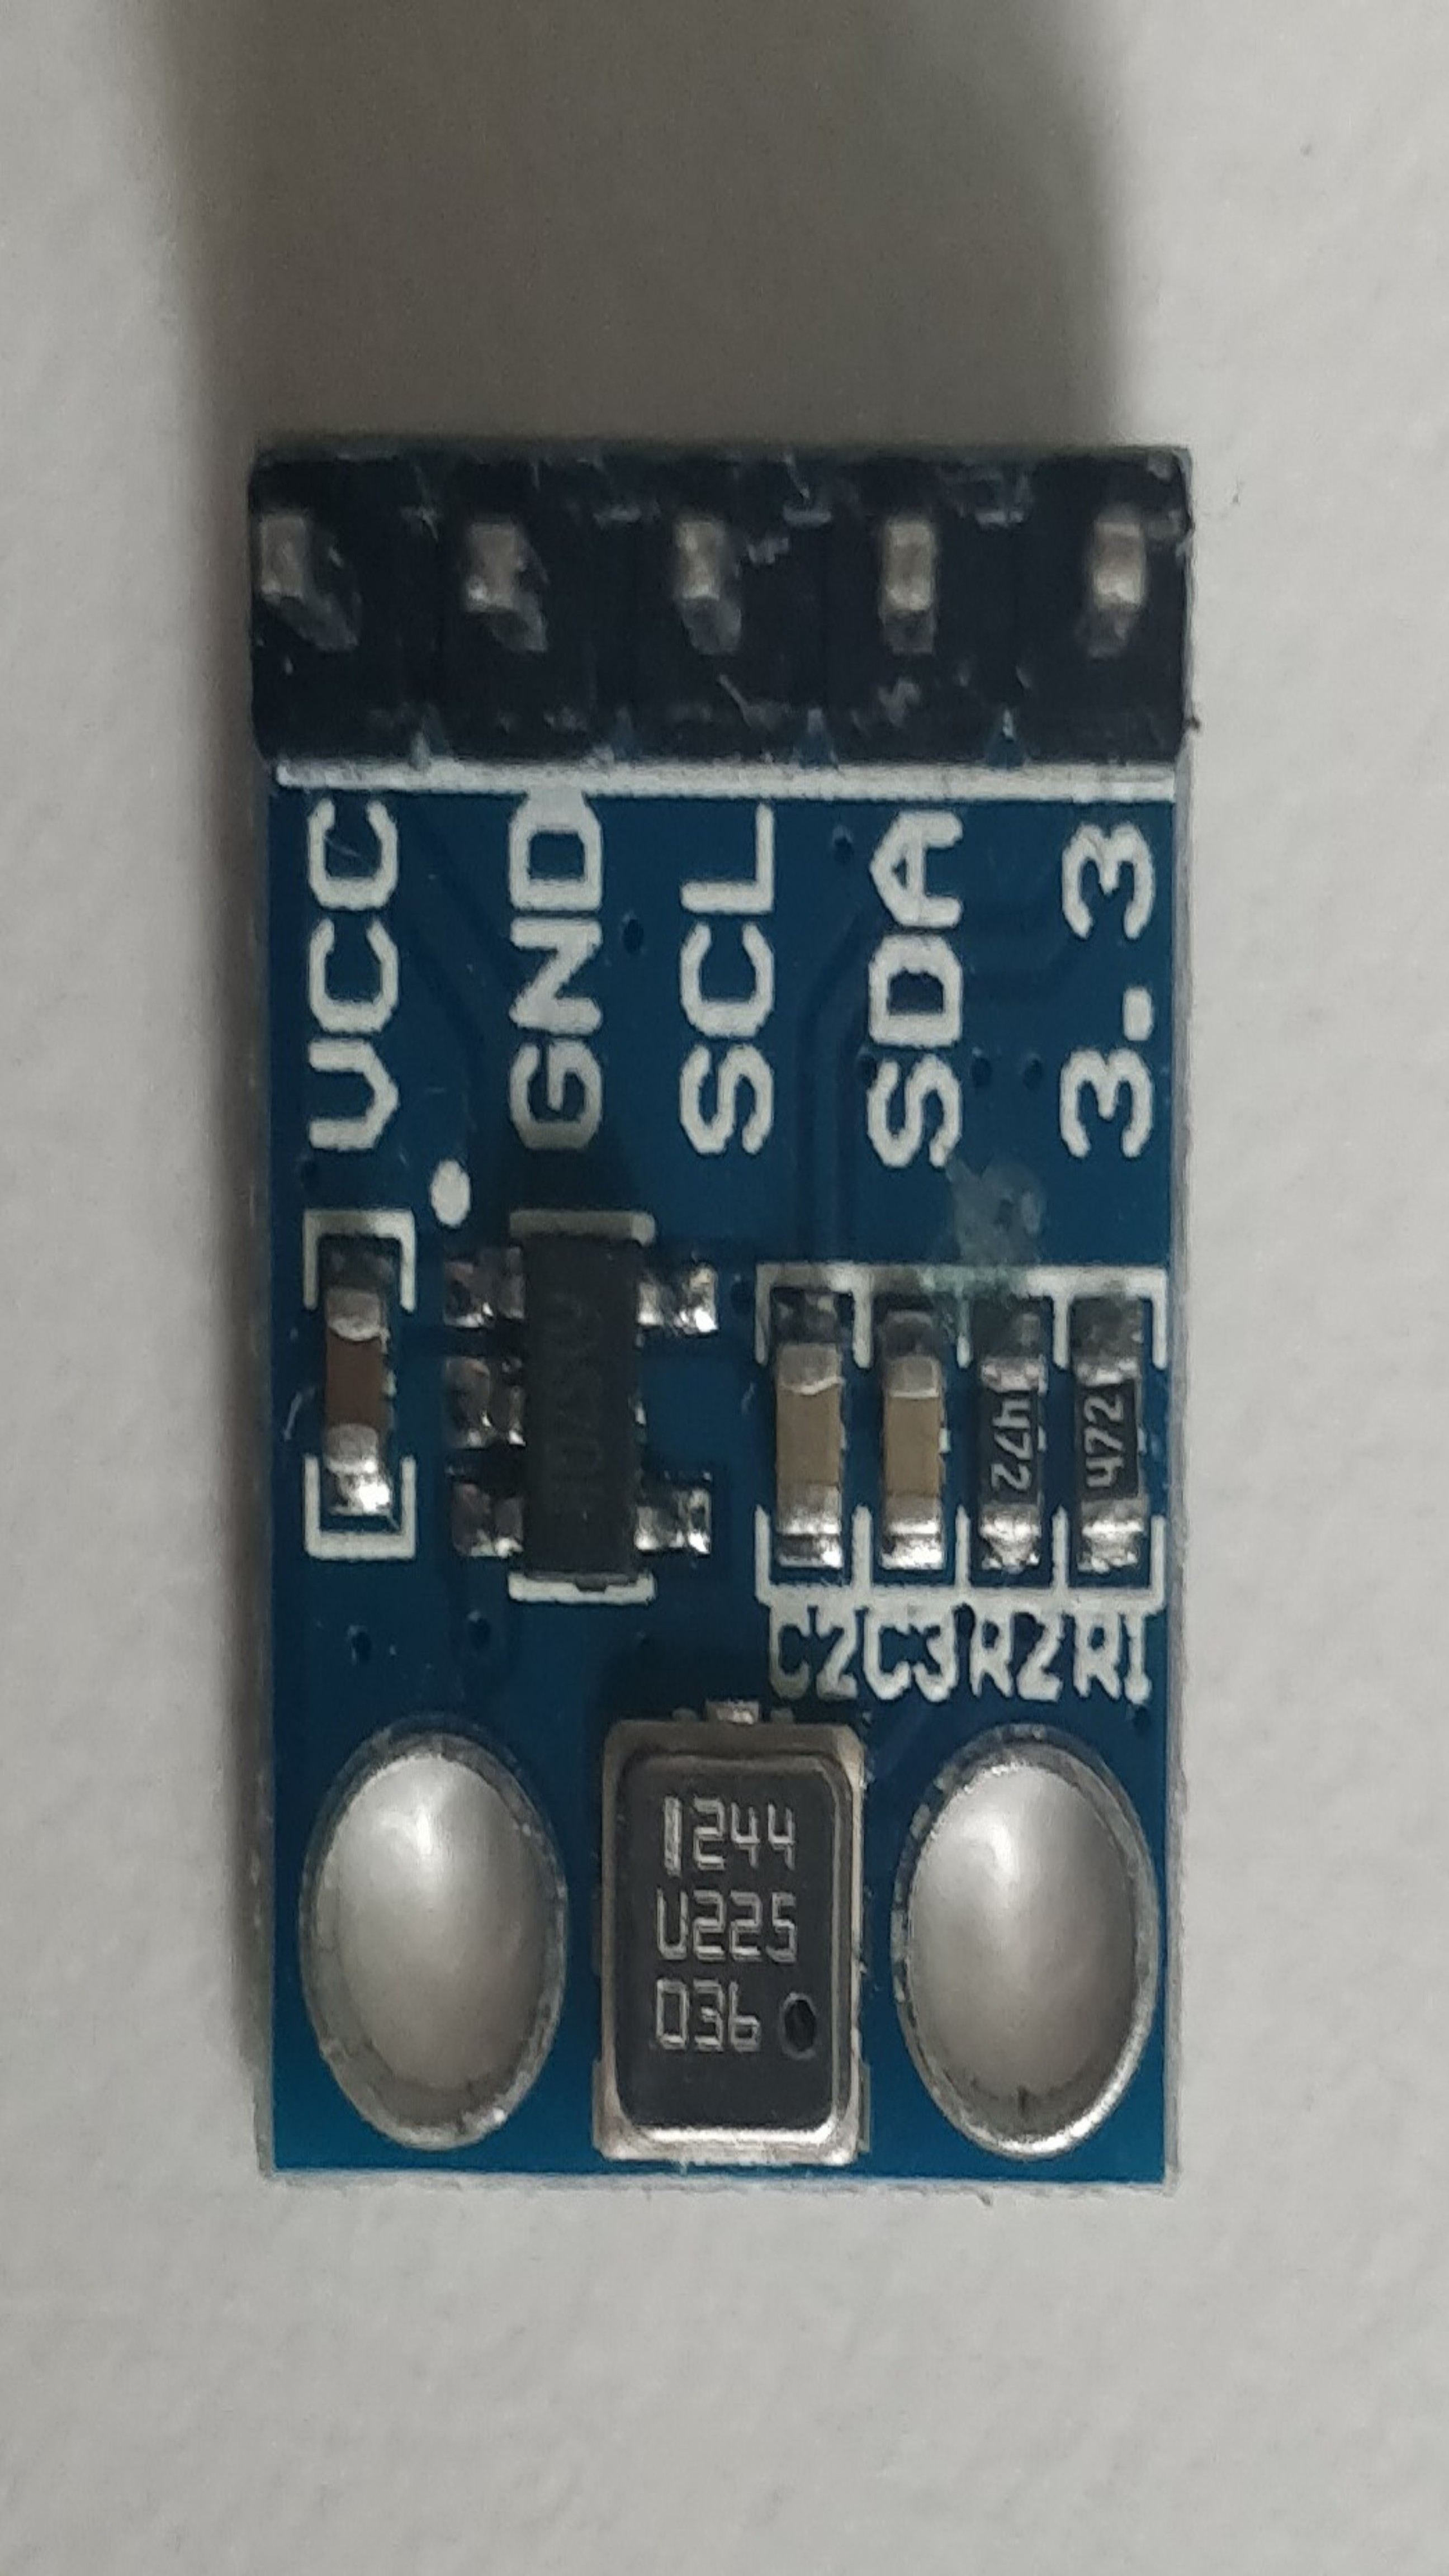
\includegraphics[scale=0.03,angle=270]{fig/pressuresensor.jpg}

\captionof{figure}[BMP180 Pressure Sensor]{BMP180 Pressure Sensor}
\label{fig:bmp180}
\end{center}
\item  Then, an ethernet wire is connected to the board and Linux laptop. Reset button is pressed on the board after flashing and "dmesg" command is executed in a Linux terminal to check the USB port to which the board is connected.
\item To launch Nuttx console, "sudo minicom -s" command is executed in Linux and USB port of the board is selected. The user needs to press enter 3 times everytime the console is launched.
\item Then in the console, "ifup eth0" is executed to enable ethernet. "ifconfig" command can be used to check IP addresses of the device and network. Then, "mount -t procfs proc" is executed to mount the file system to access the network applications.
\item The user can type "help" to see all built-in applications. The applications "publisher", "subscriber", "bmp180\textunderscore publisher", "bmp180\textunderscore subscriber", and "delay\textunderscore test" were enabled in this setup.
\item The delay\textunderscore test adds a timestamp, then publishes a message and sends to the agent and subscribes it back again. Then it adds another timestamp and calculates the difference between the initial time and final time. Hence, the delay in micro-ROS communications can be recorded. Figure 4.4 shows the overview of the delay\textunderscore test algorithm.
\begin{center}
\hspace*{-1cm}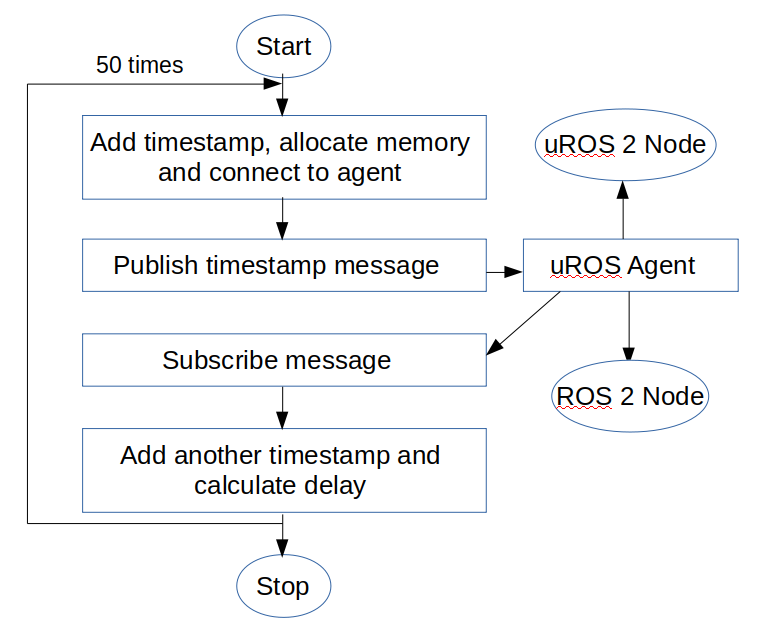
\includegraphics[scale=0.35]{fig/delay.png}

\captionof{figure}[Delay Test]{Delay Test}
\label{fig:delay}
\end{center}
\item To increase the data sizes of the messages, custom ROS messages were created and testing was repeated with message sizes of 8 bytes (an integer data size is 4 bytes), 16 bytes, 32 bytes, 64 bytes, and 128 bytes.
 
{\bfseries Note}: The firmware and agent software has to be deleted and compiled again every time the message file or algorithm is changed.

Figure 4.5 shows the complete set-up with Olimex board, ethernet, micro-USB and connection to the pressure sensor with 4 UART coloured wires.
\begin{center}
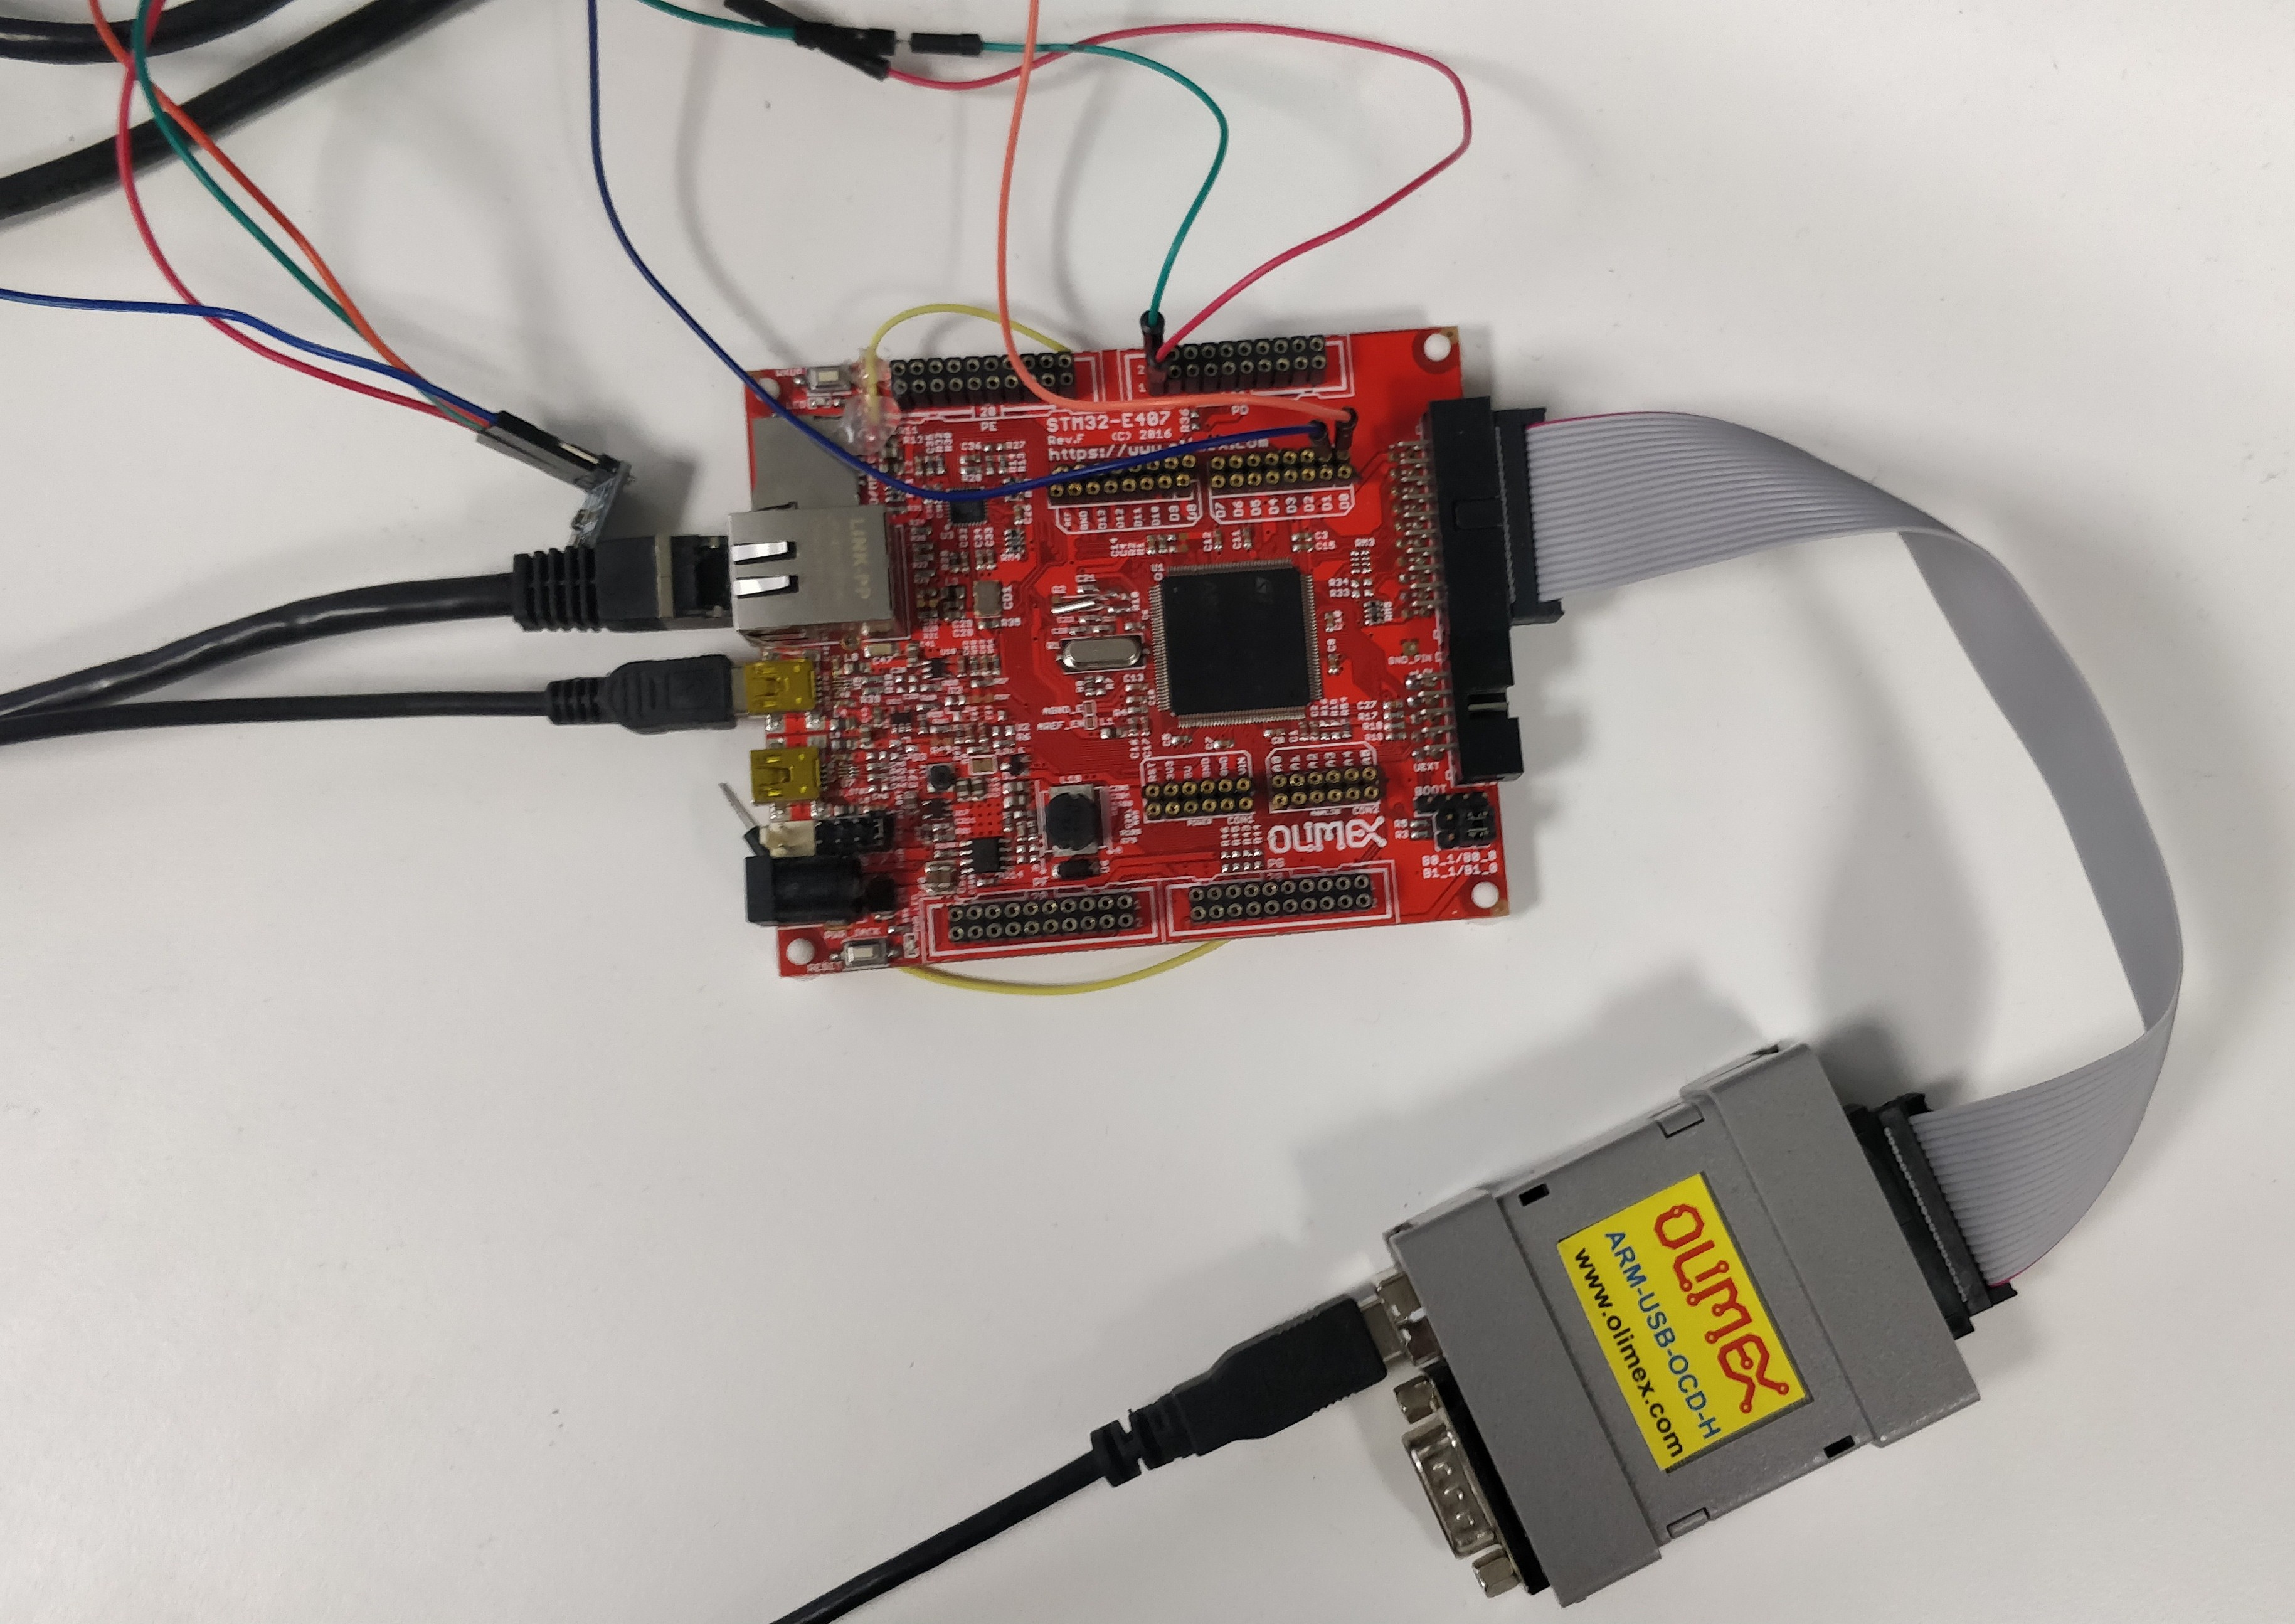
\includegraphics[scale=0.1]{fig/olimex.jpg}

\captionof{figure}[Olimex Setup]{Olimex Setup}
\label{fig:olimexsetup}
\end{center}
\item Similarly, the waveshare board was set-up. Steps 5 and 8 were skipped as pressure sensor and ethernet connection are not required. Although, if required, DP83848 ethernet to UART converter can be used to setup ethernet as well. A USB to UART converter cable was connected in the following sequence to enable serial transport of micro-ROS: 
\begin{itemize}
\item Black wire of connector to ground of the board using UART3 port
\item Green wire to RX port.
\item White wire to TX port.
\end{itemize}

Figure 4.6 shows the Waveshare MCU set-up with micro-USB cable to access the Nuttx console and 3 UART wires through which data exchange takes place.
\begin{center}
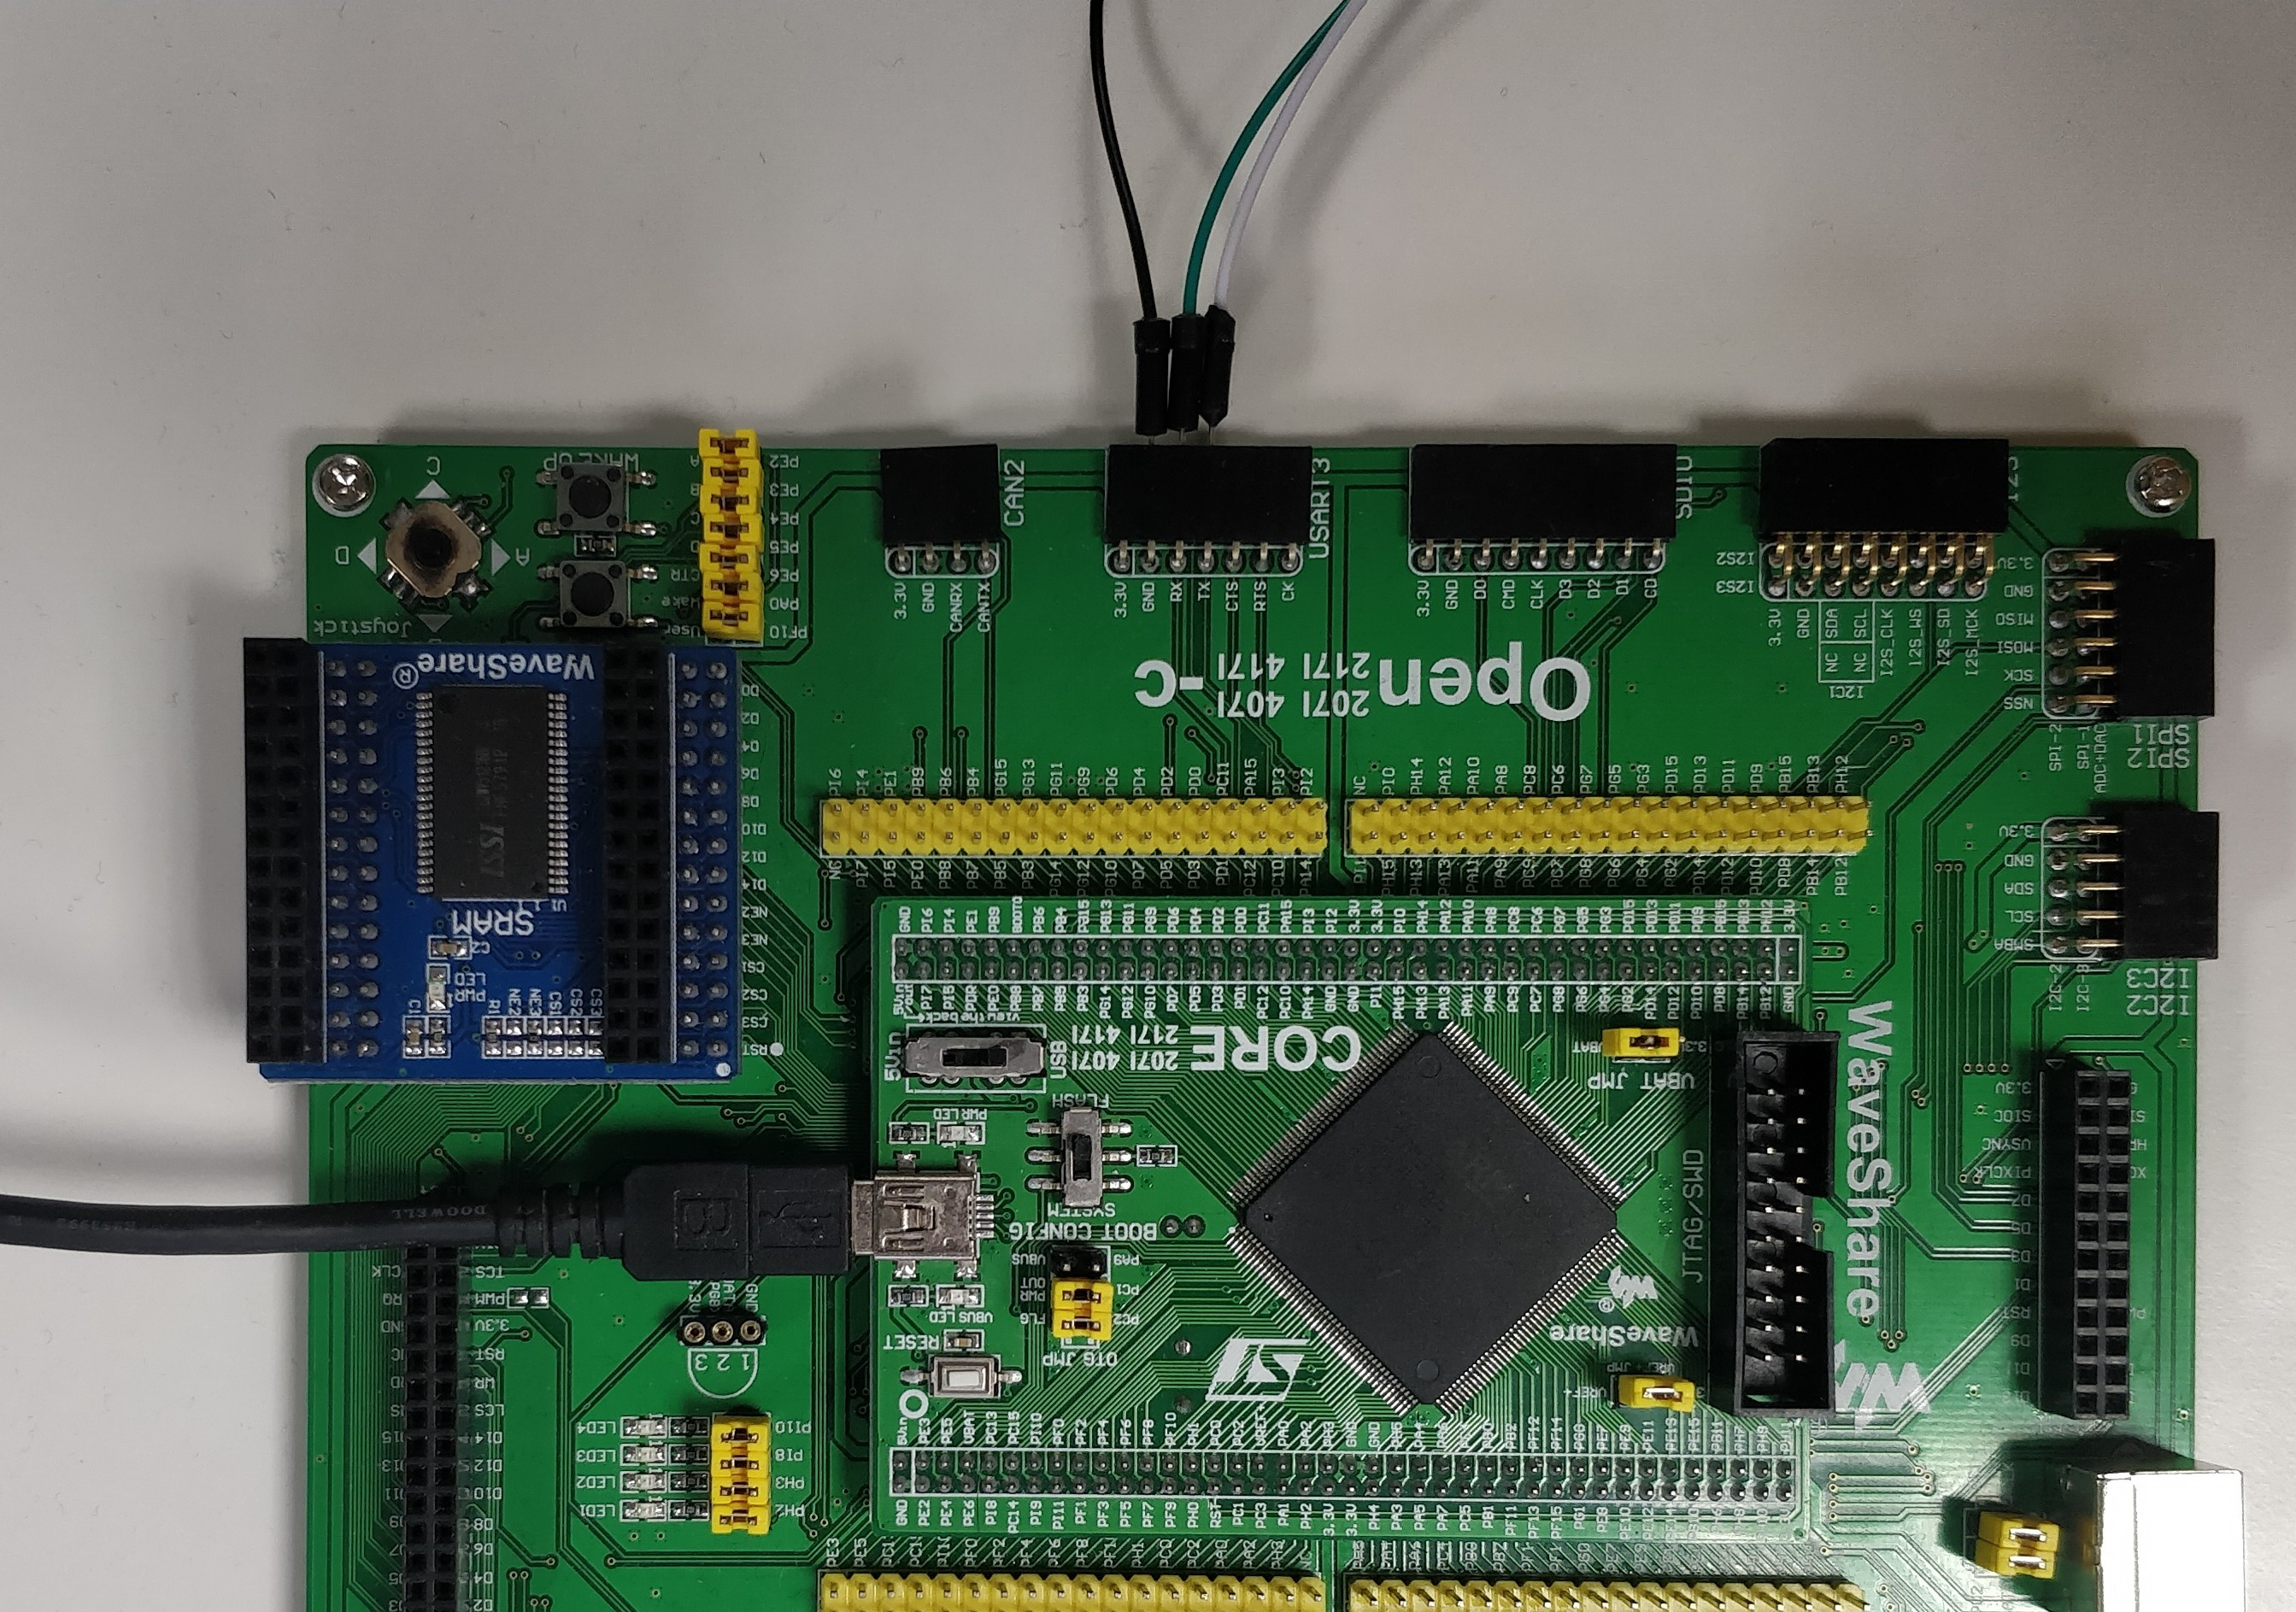
\includegraphics[scale=0.15,angle=180]{fig/waveshare.jpg}

\captionof{figure}[Waveshare Setup]{Waveshare Setup}
\label{fig:wavesharesetup}
\end{center}
\item Micro-ROS Agent was launched in another terminal in Linux. Then ROS 2 crystal environment was sourced and the micro-ROS environment was sourced. Micro-ROS agent package can be found in the install directory in "uros\textunderscore ws". Micro-ROS agent was launched with commands "./micro\textunderscore ros\textunderscore agent udp 8888" for IP connection and "./micro\textunderscore ros\textunderscore agent serial <USB port number for PL2303 driver>". 
\item Finally, the "delay\textunderscore test" application was executed in Nuttx console. "delay\textunderscore test" was executed 10 times using a loop of 50 observations in each execution and all data was recorded.
\end{enumerate}

		\chapter{Results}
			
\rofoot[\pagemark]{\pagemark}
\refoot[\pagemark]{\pagemark}
In this chapter, first the latency and jitter observations of the pendulum demo for ROS 2 Crystal and Dashing are documented and analyzed. Then, the reliability test cases with their results are mentioned and observations of micro-ROS "delay\textunderscore test" with messages of different data sizes are analyzed. In the end, some common aspects of the result data of ROS 2 and micro-ROS are discussed in detail.
		\section{Latency Analysis of ROS 2}
\vspace*{0.25cm}
In this section, the results of the inverted pendulum demo for ROS 2 Crystal and Dashing are documented, explained and analyzed.
\vspace*{0.25cm}

{\bfseries ROS 2 Crystal}
\vspace*{0.25cm}

\sisetup{math-micro=\text{µ},text-micro=µ}
In this package, the messages were sent every 1 ms. The goal of this package was to receive 1000 messages with maximum 3 \% jitter (30 \si\micro s). In this testing, 1 megabyte (MB) of memory and high real-time priority were available to the node.

\vspace*{0.2cm}
 Table 5.1 shows the output of the pendulum demo package. The package printed out minimum, maximum and mean latency values, standard deviation and number of messages received by the controller in each execution of the package. First 5 observations were without any stress on the CPU and the next 5 were with stress applied on the CPU.

\vspace*{0.2cm}
Even though minimum latency values are very low, still the mean latency is over 1 ms in 2 observations which is greater than the update rate. The maximum latency is 44.5 ms and the maximum jitter value is 33 ms which is way beyond the desired. The data exchange is not reliable as messages are lost. 
\vspace*{0.2cm}

Standard deviation values are large and constant without any stress on the CPU suggesting that there is something wrong inside the package. Also, the simulation is not continuous, the package runs for just a few seconds and displays the result. As already mentioned in section 2.5, real-time systems are tested for longer periods of time with different conditions and this package does not allow us to control the execution time of the demo. Additionally, it just states the values giving no indication of deterministic performance and jitter in the system.
It is not suitable for continuous testing of real-time parameters.
\begin{center}
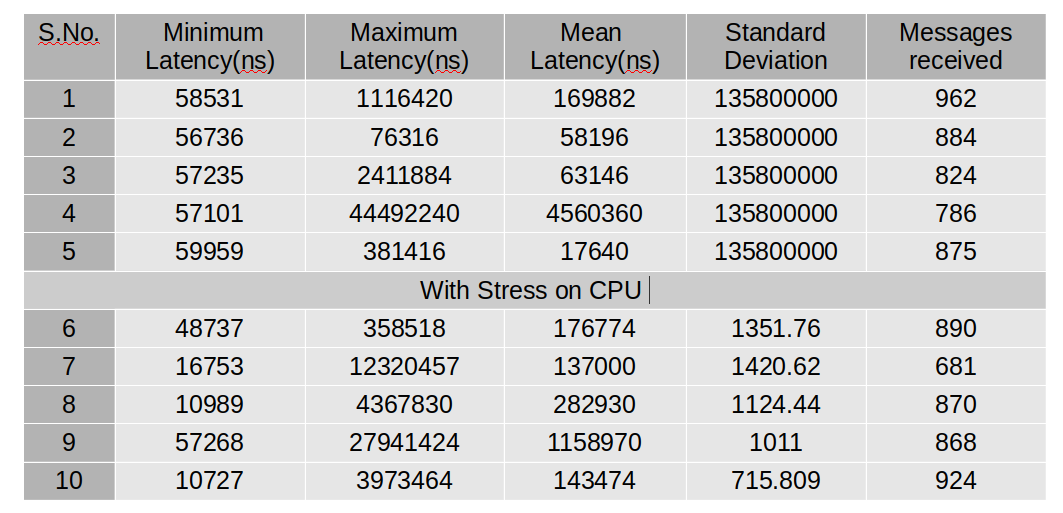
\includegraphics[scale=0.38]{fig/ros2crylatency.png}
\captionof{table}[ROS 2 Crystal Latency]{ROS 2 Crystal Latency}
\label{tab:ros2crystallatency}
\end{center}


{\bfseries ROS 2 Dashing}
\vspace*{0.25cm}

In this package, the messages were sent every 1 ms and the deadline was defined as 2 ms. 1 MB of memory and high real-time priority were available to the node.  

\vspace*{0.2cm}
Table 5.2 shows the output of this pendulum demo package. The package printed out minimum, maximum and mean jitter, and standard deviation of jitter. The jitter is continously calculated with respect to the previous update. Also, this is a continuous simulation which can be visualized. The user can also give out a disturbance signal and see the system react to it. The position of the cart was changed by an external force on it, but the pendulum did not fall down.

\vspace*{0.2cm}
The jitter and standard deviation kept increasing with time. The maximum jitter value is 80 ms.
Although, the mean jitter values close to zero and the pendulum not falling down suggest good real-time performance but the increasing standard deviation and high jitter values give us an impression that some improvements in the ROS 2 execution is required to make ROS 2 more predictable and suitable for real-time systems. It should also be taken into consideration that the Linux real-time kernel does not guarantee a hard real-time system.

\vspace*{0.2cm}
This package is suitable for testing soft real-time systems like a Linux environment and future versions of ROS 2 can be tested with it.
\begin{center}
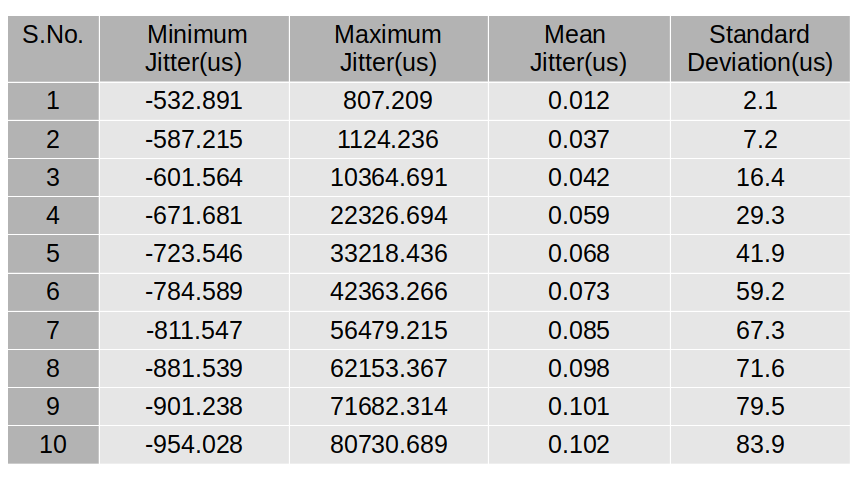
\includegraphics[scale=0.4]{fig/ros2dashjitter.png}

\captionof{table}[ROS 2 Dashing Jitter]{ROS 2 Dashing Jitter}
\label{tab:ros2dashjit}
\end{center}
		\section{Reliability of micro-ROS}
		\vspace*{0.5cm}
		Some software bugs and missing features were found during the testing:
	\begin{itemize}	
	\item Multiple microcontrollers can not be connected to a single micro-ROS Agent/Server. This is one of the important features of micro-ROS which is missing. The issue has been reported to the micro-ROS developers. Five test cases were created to test reliability:
\begin{itemize}
\item {\bfseries Case 1}: Using built-in publisher-subscriber of micro-ROS through ethernet (UDP) with one micro-ROS agent. 
Publisher was launched on the olimex board and subscriber was launched on the waveshare board. Both of them were communicating through the same IP address and port number. Message sending rate was really fast (1 ms) in this example, subscriber code was changed to receive 500 messages and then stop. \linebreak
{\bfseries Result}: Only one of the nodes worked, either publisher or subscriber.

\item {\bfseries Case 2}: Using built-in publisher-subscriber of micro-ROS through ethernet (UDP) with two micro-ROS agents with different port numbers.\linebreak
{\bfseries Result}: Only one of the nodes worked, either publisher or subscriber.

\item {\bfseries Case 3}: Using bmp180 pressure sensor and same structure of publisher-subscriber code as the built-in example through ethernet (UDP), first with one micro-ROS agent and then 2 agents with different port numbers.
Message is sent every 1 second.\linebreak
{\bfseries Result}: Both nodes were initialized at both the boards. Subscriber received very less data, for instance, it received only 2 messages while the publisher published 15 messages in the same time, therefore it is not reliable.

\item {\bfseries Case 4}: Using built-in publisher-subscriber with 1 agent through ethernet (UDP) and 1 agent through serial (UART) communication.
Data sending rate was 1 ms.\linebreak
{\bfseries Results}: Nodes were initialized, but many messages were not received by the subscriber, therefore it is not reliable.

\item {\bfseries Case 5}: Using BMP180 pressure sensor with 1 agent through ethernet (UDP) and 1 agent through serial (UART) communication.
Data was sent every 1 second. \linebreak
{\bfseries Results}: Nodes were initialized and all values were received.
\end{itemize}
\item Transport of arrays are not supported in the messages by micro-ROS. Therefore, string messages, array of numbers, or an image cannot be transported as of now. Therefore, a pressure sensor had to be used to use the standard integer message package. Also, testing of large message sizes (e.g. - image messages) could not be performed.

\end{itemize}
\section{Latency Analysis of micro-ROS}

\vspace*{0.5cm}
In this testing of delay in micro-ROS communications, sometimes the subscriber got timed out and killed the node which hampered testing. Later, it was confirmed with the micro-ROS developers that this was also a bug in the software. Due to this issue, multiple publishers and subscribers present in a single node could not be tested. Also the latencies using the UART serial communication were 15-20 ms more than the latencies using ethernet (UDP) communication because of the lag caused by the driver in the USB to UART converter. Therefore further testing was only done using ethernet. There were some promising results:
\begin{itemize}
\item The latencies in \si\micro s for 500 observations for a message size of 8 bytes is shown in figure 5.1. The least count of the board's clock was 10 ms. Deterministic performance can be observed but with multiple latency spikes.

\begin{center}
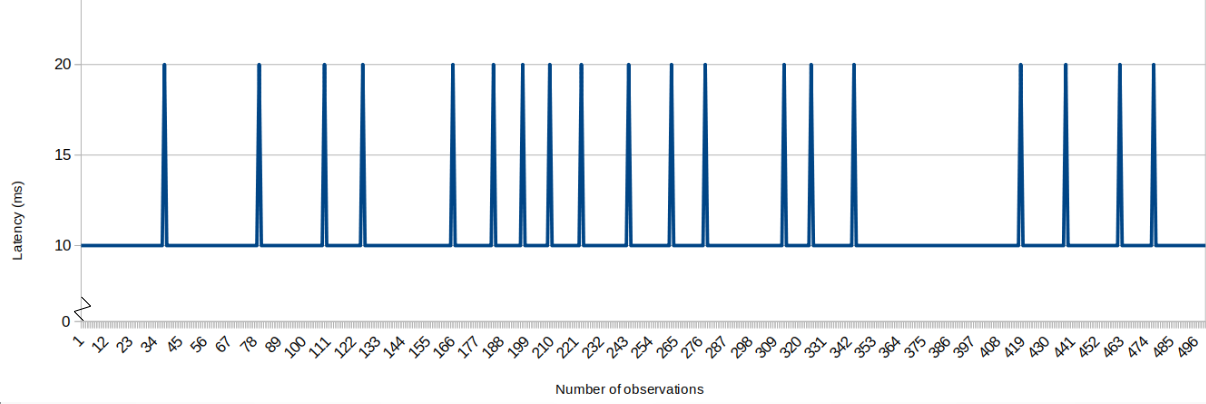
\includegraphics[scale=0.345]{fig/uros8byteles2.png}
\captionof{figure}[Micro-ROS Latencies for Data Size of 8 bytes (Least count-10 ms)]{Micro-ROS Latencies for Data Size of 8 bytes (Least count-10 ms)}
\label{fig:uros8byteles}
\end{center}

\item The latencies in \si\micro s for 500 observations for a message size of 8 bytes is shown in figure 5.2. The least count of the board's clock was changed to 10 \si\micro s for better precision. An acceptable jitter of 1 ms was defined. Figures 5.3, 5.4, 5.5 and 5.6 show the observations of the delay test with message sizes of 16 bytes, 32 bytes, 64 bytes, and 128 bytes respectively. There were multiple instances of overruns in each case.
\nomenclature{MB}{Megabyte}
\nomenclature{ns}{Nanoseconds}
\nomenclature{ms}{Milliseconds}
\nomenclature{\si\micro s}{Microseconds}
\begin{center}
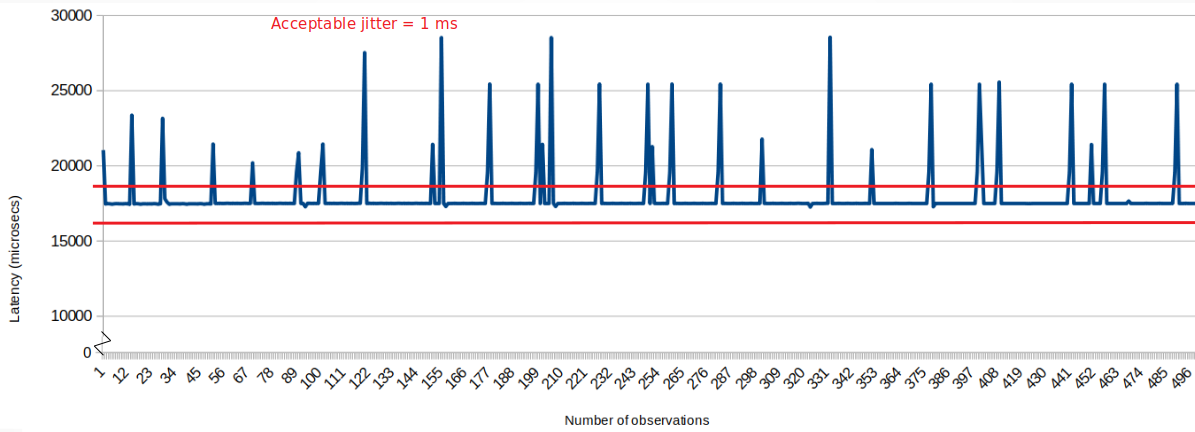
\includegraphics[scale=0.34]{fig/uros8byte2.png}

\captionof{figure}[Micro-ROS Latencies for Data Size of 8 bytes (Least count-10 \si\micro s)]{Micro-ROS Latencies for Data Size of 8 bytes (Least count-10 \si\micro s)}
\label{fig:uros8byte}
\end{center}


\begin{center}
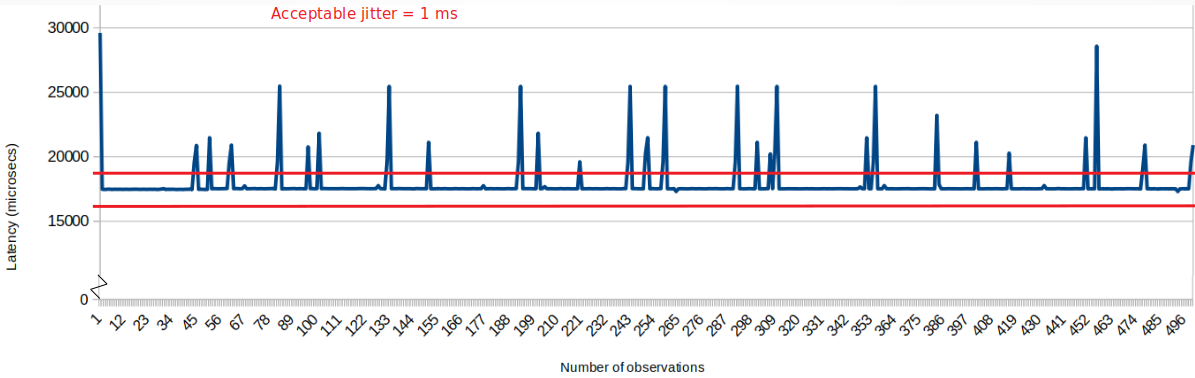
\includegraphics[scale=0.34]{fig/uros16byte2.png}

\captionof{figure}[Micro-ROS Latencies for Data Size of 16 bytes (Least count-10 \si\micro s)]{Micro-ROS Latencies for Data Size of 16 bytes (Least count-10 \si\micro s)}
\label{fig:uros16byte}
\end{center}

\begin{center}
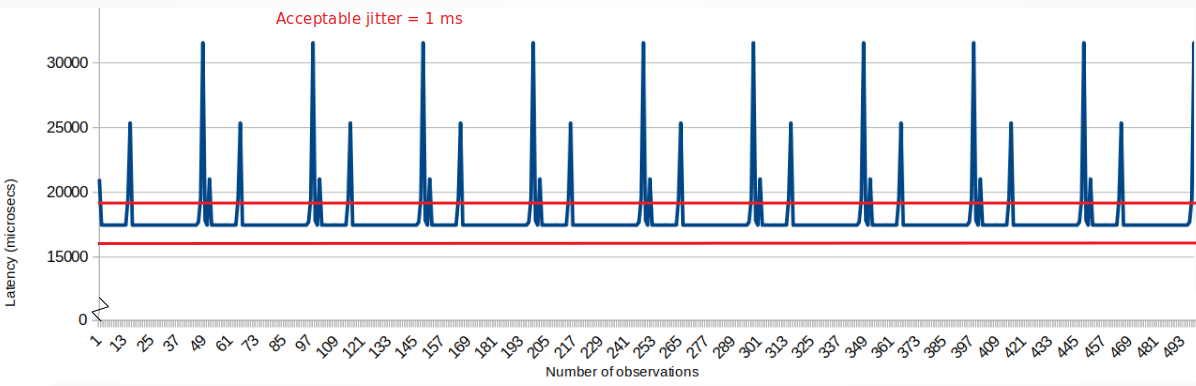
\includegraphics[scale=0.34]{fig/uros32byte2.png}

\captionof{figure}[Micro-ROS Latencies for Data Size of 32 bytes (Least count-10 \si\micro s)]{Micro-ROS Latencies for Data Size of 32 bytes (Least count-10 \si\micro s)}
\label{fig:uros32byte}
\end{center}

\begin{center}
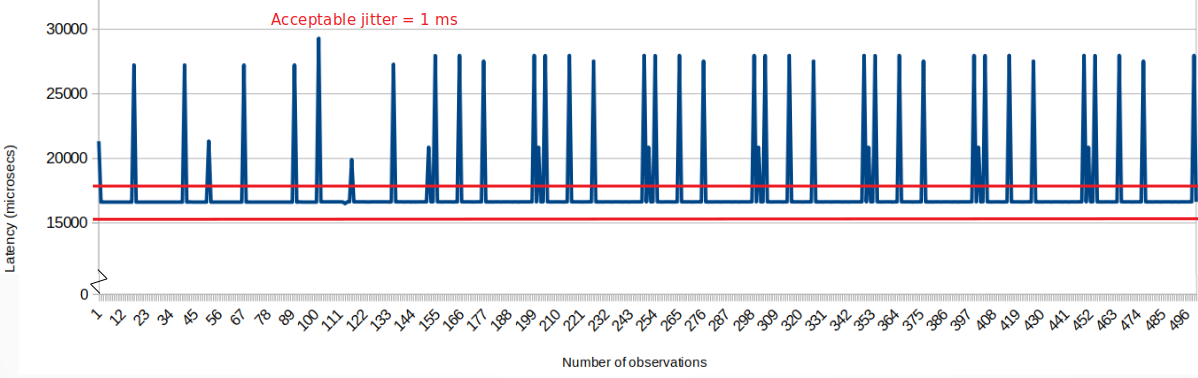
\includegraphics[scale=0.34]{fig/uros64byte2.png}

\captionof{figure}[Micro-ROS Latencies for Data Size of 64 bytes (Least count-10 \si\micro s)]{Micro-ROS Latencies for Data Size of 64 bytes (Least count-10 \si\micro s)}
\label{fig:uros64byte}
\end{center}

\begin{center}
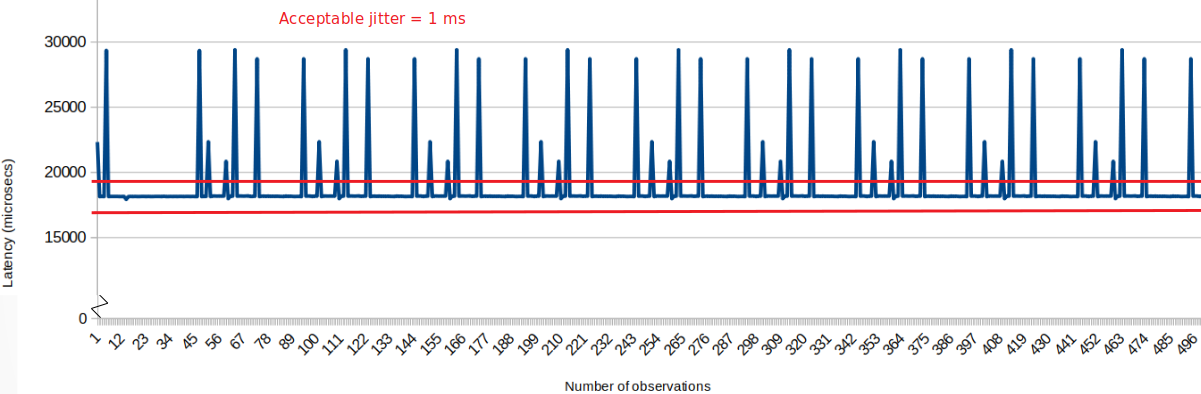
\includegraphics[scale=0.34]{fig/uros128byte2.png}

\captionof{figure}[Micro-ROS Latencies for Data Size of 128 bytes (Least count-10 \si\micro s)]{Micro-ROS Latencies for Data Size of 128 bytes (Least count-10 \si\micro s)}
\label{fig:uros128byte}
\end{center}
\end{itemize}
{\bfseries Analysis}


\vspace*{0.5cm}
From the line graphs, deterministic performance of the micro-ROS LET Executor is observed. Many latency spikes outside the range of acceptable jitter were also observed. In table 5.3, mode latency, maximum jitter, mean jitter, and number of overruns with respect to different data sizes are shown. Low mean jitter values and mode latencies suggest good real-time performance with a RTOS. But, these maximum jitter values and multiple overruns are not suitable for a hard real-time system. Also, it can be observed that the mean jitter value and instances of overruns increase with increase in message data size.
\begin{center}
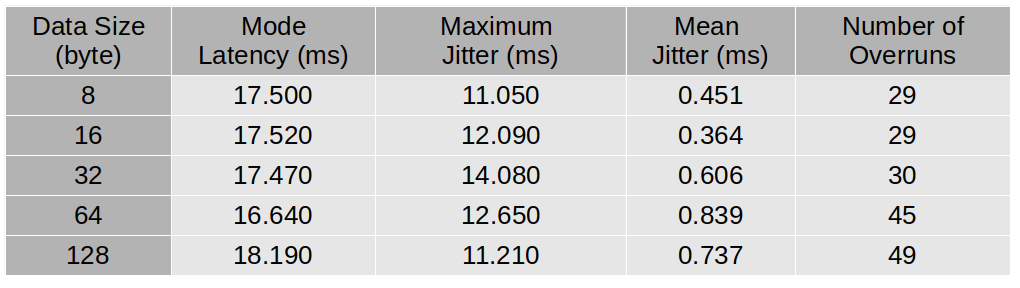
\includegraphics[scale=0.4]{fig/urosfinaldata.png}

\captionof{table}[Micro-ROS Results]{Micro-ROS Results}
\label{tab:urosfinaldata}
\end{center}
		
		\section{Discussion and Comparison}
		\vspace*{0.25cm}
	Since, the packages and ways of testing for ROS 2 Crystal, ROS 2 Dashing and micro-ROS (ROS 2 Crystal) are different. The results should not be compared between them. However, we can still determine some common aspects of their results.
	
	\vspace*{0.25cm}
	ROS 2 Crytal pendulum demo is not a continuous simulation and does not show good real-time performance. This package is not suitable for testing real-time capabilities as it just states out the values and deterministic performance cannot be seen from these values. The mean latency values are low but the large standard deviation and maximum latencies are not good for a real-time system. Also, there is a loss of data which increases when stress is applied. 
	\vspace*{0.25cm}
	
	ROS 2 Dashing pendulum demo provides more data to determine the real-time performance and also offers a continuous visual simulation in the RViz package. Mean jitter values were very low but they kept on increasing with time. Also, the high maximum jitter and standard deviation values suggest that there is some improvement needed to make the execution more deterministic. It also gives an impression that with some fine-tuning and improvements in the ROS 2 standard executor, the software can be configured for a soft or firm real-time system. However, this package should be tested with a RTOS. The main issues related to real-time performance have been identified by users of ROS 2 and they are working along with ROS 2 developers to improve the real-time performance.
	
	\vspace*{0.25cm}
	There is also an alternative to the standard ROS 2, which is micro-ROS specifically targeting embedded board and real-time applications. However, extensive development of micro-ROS is required to provide reliable software. The testing of this software was only partially successful.  Deterministic behaviour of the LET executor and low mean jitter values were observed. But, high maximum jitter values and multiple overruns were also observed. Even though micro-ROS runs on a RTOS, the agent still requires a Linux environment which is not real-time safe. The agent is a core element of the communication structure and running it on a non RTOS will have a negative impact on the real-time performance of micro-ROS. Also, multiple numbers of publishers and subscribers could not be launched due to a software bug and stress could not be applied to the MCU. The C++ executor is still a challenge and is under development. Further testing of micro-ROS under different conditions and through different ways can only be done, once the limitations in the software are removed. 
		\chapter{Conclusion}
			
\rofoot[\pagemark]{\pagemark}
\refoot[\pagemark]{\pagemark}
The investigation in the real-time performance of the standard ROS 2 stack suggest that it still requires improvement and further development in some of its packages to make it suitable for a real-time system, especially for hard real-time applications. Currently, it only seems suitable for soft real-time systems as it offers low latency values and mean jitter values close to zero in the case of the Dashing version. Also, the underlying DDS middleware can be fine-tuned for better real-time performance, but this needs to be further investigated. Based on the research by ROS 2 developers, Bosch and Nobleo, the issues with the software have been identified and some special features related to real-time systems might be offered in the upcoming versions of ROS 2. The inverted pendulum demo can be used as a standard platform to test the upcoming versions. But, with its variety of libraries, ROS 2 can definitely be used for automotive applications as it was observed with the ADAS simulator.

\vspace*{0.25cm}
micro-ROS offers deterministic behaviour on a RTOS and is more suitable than the standard ROS 2 stack for a real-time system. But, it requires extensive and fast development to offer its users a real-time safe and reliable software. Still, the limitations of this software remain to be tested as there are a lot of bugs and their development needs to integrate with the standard ROS 2 stack. Also, the micro-ROS agent dependency needs to be eliminated because it runs on an environment which is not real-time safe. Unless these issues are resolved, mico-ROS is not suitable for automotive applications because the versatile libraries of ROS 2 cannot be used at this stage with the current micro-ROS core execution packages.


\section{Future Scope}
\vspace*{0.2cm}
The shortcomings of ROS 2 suggest that there is extensive development still needed to make ROS 2 suitable for real-time systems especially for automotive applications.
 Future versions of ROS 2 can be tested with the inverted pendulum demo and the results can be compared with that of Dashing. Investigation on configuration and fine-tuning of DDS by different vendors for better real-time performance is also required.
 \vspace*{0.15cm}
 
 Real-time applications are best tested in a dynamic environment over a long period of time. Testing of inverted pendulum demo can be done with micro-ROS and RTOS when the C++ executor becomes available. A physical hardware setup of an inverted pendulum for testing with micro-ROS can also be developed.
Real-time testing of image messages using a camera sensor and micro-ROS can also be done as image processing is important in the field of automated driving.
ROS 2 can also be compared with other software in the same testing environment. For example, the driverless Formula student racing team at the Ravensburg Weingarten University can compare the performance of different software with a parameter like brake distance measurement after defining a physical trigger point to apply the brakes or observe the deviation in the path the car takes on the track over multiple laps.

		\addcontentsline{toc}{chapter}{List of Figures}
	\listoffigures
	\addcontentsline{toc}{chapter}{List of Tables}
	\listoftables
		
		\addcontentsline{toc}{chapter}{Bibliography}
\bibliographystyle{ieeetr}		
\bibliography{thesis}





\end{document}
